\documentclass[article,type=msc,colorback,accentcolor=tud9c, 11pt]{tudthesis}
\usepackage{setspace}
\usepackage{multirow}
\usepackage[normalem]{ulem}
\useunder{\uline}{\ul}{}
\usepackage{fancyhdr}
\usepackage{amsmath}
\usepackage{hyperref}
\usepackage{float}
\usepackage{longtable}
\usepackage{enumerate}
\usepackage{enumitem}
\usepackage[figuresright]{rotating}
\usepackage{adjustbox}
\usepackage{array}
\newcolumntype{R}[2]{%
    >{\adjustbox{angle=#1,lap=\width-(#2)}\bgroup}%
    l%
    <{\egroup}%
}


\setlist[description]{leftmargin=1.5cm,labelindent=0.5cm}

\newcommand*\rot{\multicolumn{1}{R{45}{1em}}}
\hypersetup{
    colorlinks,
    citecolor=black,
    filecolor=black,
    linkcolor=black,
    urlcolor=black
}
\numberwithin{equation}{section}

\setstretch{1.5}

\newcommand{\getmydate}{%
  \ifcase\month%
    \or Januar\or Februar\or M\"arz%
    \or April\or Mai\or Juni\or Juli%
    \or August\or September\or Oktober%
    \or November\or Dezember%
  \fi\ \number\year%
}

\renewcommand*\contentsname{Table of Content}



\begin{document}
  \thesistitle{Related Articles Discovery in Large Corpora}%
    {}
  \author{Ziyang Li}
  \birthplace{Tianjin, China}
  \referee{Prof. Dr. Iryna Gurevych}{Nils Reimers}
  \department{Fachbereich Informatik}
  \group{Ubiquitous Knowledge Processing}
  \dateofexam{\today}{\today}
  \makethesistitle
  \affidavit{Ziyang Li}
  
  \pagenumbering{roman}
  \setcounter{page}{1}
  \tableofcontents
  \newcommand{\iSP}{\textit{SP }}
\newcommand{\iSE}{\textit{SE }}
\newcommand{\iST}{\textit{ST }}
\newcommand{\iSS}{\textit{SS }}
\newcommand{\ifull}{\textit{full }}
\newcommand{\icommon}{\textit{common }}
\newcommand{\ititle}{\textit{title }}
\newcommand{\icontent}{\textit{content }}
\newcommand{\isummary}{\textit{summary }}
  \clearpage
  
  \pagenumbering{arabic}
  \setcounter{page}{1}
  \section{Introduction}

As we read a piece of news or report, we often would like to know extra information about the news, probably the background, the recent progress or the other news on the same topic. Many online newspaper providers provide extended reading material after articles. ZEIT Online is a good example. The articles in the ZEIT Online, contain at the end of each article two hyperlinks to further articles that are on the same topic. Theses related articles enable the user to acquire more information of knowledge on the topic of interest. At the moment those articles are selected by the authors manually. However, this imposes several issues. First, there are about $400,000$ articles in the corpus. It is quite a challenge for the author to find the suitable articles from the tremendous corpus. Second, the author selects related articles normally immediately after the article is written. Therefore, the selected related articles must be released previously and be never updated once they are selected. The reader often exactly wants to obtain the recent information of the topic, after he reads a previous article. Third, the assignment of selection requires the knowledge of the topic and hence the knowledge base of the author have the important influence of the availability of the selection.

In this thesis, the kernel objective is to evaluate how such a process could be automated. In other words, we attempt to find an approach to replace the manual selection by a fully automated process. The first issue is how and why the author selects an articles as related to the target article. We do not know the exact process of human thinking.  However, we can consider the process simplified as a process of machine. Assume that a target article requires related articles. Every candidate article is compared with the target article and a score which refers to the probability of being related article is then computed. Finally, articles with the highest scores are selected as the related articles to the target. 

Each article in the ZEIT corpus is a semi-structured instance. One instance contains structured components which are called as meta-data, such as ``author'' and ``release time'', and unstructured components which are called as text fields, such as \ititle{} and \icontent{}. One issue of the research is how to make full use of such data to improve the system usability as much as possible. The most important field of an article is the text fields including \ititle{}, \isummary{} and \icontent{}. We cope with the text fields with Semantic Textual Similarity (STS) methods, e.g. Jaccard and \tfidf{}. The models of STS methods are learned from the entire corpus. After that, the text fields are transformed to structured data, such as vectors and the scores of similarity are then computed. The scores become the measure, such that all candidate articles are ordered and selected. The score is generated so far only by one STS method over one text field. The another issue is hence how to compute overall scores which are generated by the good combination of the components of articles. We consider the comparison between two articles as a set of comparisons between corresponding components of the articles. The relatedness between two articles is therefore represented as a series of scores. We use the supervised methods to treat the scores as features of an article-pair and compute the single output value as the relatedness score of the article-pair.

\clearpage

We now give the overview of the main content of the work as follows:
\begin{description}
    \item[Section 2] The term ``Semantic Textual Similarity (STS)'' is interpreted at first and several existing STS methods which belong to string-based algorithms and vector space models are introduced and their advantages and disadvantages are discussed. The three approaches of machine-learned ranking are summarized. In the end of the section, the research questions are formulated.
    \item[Section 3] The structures of ZEIT corpus and articles are described and the related-graph which illustrates the relationship of articles is defined. After understanding the structure of corpus, the task of the research and the evaluation methods are given. 
    \item[Section 4] First, the feasibility and challenge of the system are discussed. The architecture of the system is described. Then we design two experiments to evaluate the system in the static case and in the dynamic case, respectively. 
    \item[Section 5] The results of the both experiments are given and analysed in terms of effectiveness and efficiency. The best STS methods for every different text field of articles are selected by considering both of effectiveness and efficiency. In the end of this section, we discuss several types of false predictions by way of examples.
    \item[Section 6] In the experiments in section 5, only the STS methods are evaluated. In this section, we apply the supervised methods for improving the availability of the system. The supervised methods combine the scores of the STS methods over specific text fields and the relevance scores of meta-data. Finally, the system using logistic regression has the best precision of $63.4\%$.
    \item[Section 7] This section concludes the thesis with a summary and suggestions for future work.
\end{description}
  \clearpage
  %!TEX root = <../index.tex>
\section{State of Art}
\label{sec:2}

In this chapter the common methods to calculate similarity between documents are summarized. The methods are usually categorized into two major classes, which are corpus-based and knowledge-based measures. Corpus-based measures try to calculate the value of similarity between documents using information exclusively extracted from large corpora. Normally, the corpora is used both for generating necessary knowledge (e.g. word2vec) and as input data for training models. Meanwhile, the knowledge derived from other resource, e.g. Wikipedia, New York Times, is drawn into the initializing of building models in knowledge-based measures. In our case, the corpus-based measures is preferred rather than knowledge-based measures. The reasons are briefly explained as follows. Firstly, the existent knowledge-based measures are more suitable in the field of word similarity, e.g. \cite{jiang1997semantic}, \cite{strube2006wikirelate} and \cite{Agirre2009ta}, but they are relatively weak for dealing with documents or paragraphs. The second viewpoint is that the prior knowledge has less relevance to the target corpus. The importance and meaning of a word or phrase could be different in difference resource, so that the knowledge from other resource could not interpret identical words in a specific corpus.  Furthermore, the knowledge-based measures have relatively unsatisfactory performance in case of dealing with the considerable number of Out of Vocabulary (OOV) words, whereas exactly compound words and inflection are ubiquitous in German.

In the following subsection, the traditional approaches of semantic text similarity are introduced. After that, a few of important measures of Vector Space Model (VSM) are described. The third part focuses on a short review of existent recommendation systems. The section concludes with a formulation of the research questions. 

\subsection{Traditional STS Methods}
\label{sec:2.1}

\cite{bar2013composite} proposes a classification schema which categorizes the measures into \textit{compositional measures} and \textit{non-compositional measures}. In short, \textit{compositional measures} treat documents as a sequence of words and compute document similarity by aggregating pairwise word similarity.  \textit{Non-compositional measures} regard a document as an entirety and represent it using a model. The overall document similarity is computed by comparing the representations. One of \textit{compositional measures}, introduced in \cite{islam2008semantic} and three \textit{non-compositional measures}, called LCS, GTS, Jaccard Coefficient respectively, are described as follows.

\subsubsection{Longest Common Substring/Subsequence}

Longest common substring is based on a basic idea that document is treated as sequence of characters and are compared to each other. The similarity between two texts $t_1$ and $t_2$ is:

\begin{equation}
    sim_{LCS}(t_1, t_2) = 1 -  \frac{l(t_1) + l(t_2) - 2 \cdot l(lcs(t_1, t_2))}{l(t_1) + l(t_2)}
\end{equation}

where the length $l$ of the longest contiguous character sequence $lcs$ is shared between the two texts. Moreover, longest common subsequence overcomes the limitation of continuousness. 

The kind of measures have the drawbacks. One of them is that the measures do not utilize any semantic process, while the measures cannot use any optimization method, so that the operating efficiency is in a low level. Assumed there are $d$ documents in the corpora, average $\overline{w}$ words for each document, and average $\overline{c}$ characters for each word, the time complexity of lcs is $O((d \cdot \overline{w} \cdot \overline{c})^2)$. These drawback occur also in GST, which is drawn in next part. 

\subsubsection{Greedy String Tiling}

Greedy string tiling is implemented by \cite{wise1993string}. The purpose is to detect plagiarism in programming assignment of students. The algorithm works by searching for matches of a maximum-length marking them and continuing the search ignoring marked tokens. Therefore, this method is relatively insensitive the order of words. It makes more sense for similarity computing than LCS. However, the time complexity is worse than LCS. It will be  $O(d^2 \cdot (\overline{w} \cdot \overline{c})^3)$ in the worst case. Taking into consideration of a reasonable efficiency, this method is not used in our experiments.


\subsubsection{\cite{islam2008semantic}}

\cite{islam2008semantic} introduces an extension of longest common subsequence, that computes not only the scores of lcs ($v_1$), but also the scores of maximal consecutive longest common subsequence at character 1 ($v_2$) and at character n ($v_3$). The overall score of similarity is the weighted mean of the three scores, mathematically, $sim = w_1v_1 + w_2v_2 + w_3v_3$, where $w_1 + w_2 + w_3 = 1$. 

The above described three measures regard documents as sequences of characters, so that they are not able to represent the latent relatedness of documents and they are no longer in force when they deal with long (and with multiple semantics) documents. Moreover, considering the operating efficiency these measures make sense only for short information such as title and summary of documents. 


\subsubsection{N-gram Models and Jaccard Similarity Coefficient}

From the viewpoint of n-gram models, the elementary unit of documents is not isolated words but combinations of $n$ words, where n equals 2 or 3 typically. N-gram models provide a basic processing idea, that most measures can utilize n-gram models as a part of the workflow, in order to obtain the (probabilistic) association between a word and $n-1$ words as predecessor thereof. One simple and intuitionistic measure is Jaccard similarity coefficient \cite{bank2008calculating}. For two documents $t_1=\{w^1_1, w^2_1, \cdots, w^{|t_1|-n+1}_1\}$, $t_2=\{w^1_2, w^2_2, \cdots, w^{|t_2|-n+1}_2\}$, Jaccard similarity coefficient is defined as the size of the intersection divided by the size of the union. Formally,

\begin{equation}
    sim_{jaccard}(t_1, t_2) = \frac{|t_1 \cap t_2|}{|t_1 \cup t_2|} = \frac{|t_1 \cap t_2|}{|t_1| + |t_2| - |t_1 \cap t_2|}. 
\end{equation}


\subsection{Vector Space Model}
\label{sec:2.2}

The idea of VSMs is to represent a document composed of a word sequence of an uncertain or infinite (e.g. data stream) length as a point in a vector space of a finite and determinate high-dimension. Computing the similarity of two documents $t_1$, $t_2$, is accordingly transformed as computing the similarity of the corresponding vectors $\mathbf{v_1}=(v_1^1, \cdots, v_1^s)$, $\mathbf{v_2}=(v_2^1, \cdots, v_2^s)$. The most common method is to compute $cosine$ similarity:

\begin{equation}
    sim_{cos}(t_1, t_2) = \frac{\mathbf{v_1} \cdot \mathbf{v_2}}{|\mathbf{v_1}| \cdot |\mathbf{v_2}|} = \frac{\sum_{i=1}^s v_1^i \cdot v_2^i}{\sqrt{\sum_{i=1}^s (v_1^i)^2} \cdot \sqrt{\sum_{i=1}^s (v_2^i)^2}}
\end{equation}

The $cosine$ similarity of two documents ranges from 0 to 1, when all components thereof are non-negative, e.g. in the tf-idf model, while it will rang also from -1 to 1 without the above non-negative requirement, e.g. in topic models. A variant $cosine$ similarity is so-called Pearson correlation, where vectors are normalized by subtracting the vector means $\mathbf{\overline{v}}$.  Mathematically, 

\begin{equation}
    sim_{pearson}(t_1, t_2) = \frac{(\mathbf{v_1-\overline{v}}) \cdot (\mathbf{v_2-\overline{v}})}{|\mathbf{v_1-\overline{v}}| \cdot |\mathbf{v_2}-\mathbf{\overline{v}}|}
\end{equation}

Another measure to indicate the similarity of vectors is to compute the distance, such as Euclidean distance and Manhattan distance. In this kind of similarity measure, vector normalization must be taken into account. One typical method is to make the norm of vectors as 1, so that documents of different length are treated in the equality. 

\begin{equation}
    sim_{euclidean}(t_1, t_2) = 1 - \frac{\sqrt{\sum_{i=1}^s (v_1^i-v_2^i)^2}}{\sqrt{\sum_{i=1}^s r^2}} ,
\end{equation}
where $r$ is the value range of components of vectors.

VSMs can be classified as term-weighted models and topic-weighted models according to different methods of representing. In following sections we will introduce two common measures of these two types respectively and discuss their advantages and challenges. 

\subsubsection{Bag-of-Words and \textit{tf-idf} Model}

The bag-of-words (BoW) model is a simplest term-weighted vector space model. The vector of a document is composed of the frequency of occurrence of all words in the vocabulary. The dimension of BoW vector therefore is equal to the size of the vocabulary which is normally generated using the entire corpus. The BoW model has a crucial lack that some words occur in the most documents frequently, such as ``go'', ``buy'', ``play'' in English. After normalization, these words will occupy the dominating position and the weight of other words will be	insignificant. Quite the opposite, words, which occur infrequently in the corpus and relatively repeatedly in a cluster, make more sense in the specific context or topic than the common words. 

From this view point, term-frequency-inverse-document-frequency (\textit{tf-idf}) exhibits the importance to provide the meaning or the characteristic in a specific document but not frequency itself of words. The idea contains of two parts. On one side, the metric \textit{tf} indicates how frequent the current word is in the target document. On the other siede, the metric \textit{idf} exhibits the scarcity of the word in the entire corpus. Given a document $d$ from the corpus $D$ and an arbitrary word $w_i$ in the vocabulary, 

\begin{equation}
    tfidf(w_i, d) = tf(w_i, d) \cdot log_2(\frac{|D|}{df(w_i, D)}), 
\end{equation}
where \textit{tf} is the number of occurrences of $w_i$ in $d$, and \textit{df} is the number of documents containing $w_i$. 

In both of BoW and \textit{tf-idf} models, the representation of documents is sparse vectors, of which in average more than 90\% components are zero,  because the vocabulary size is about 10k\textasciitilde 30k and each document has typically 300\textasciitilde 3k words. Furthermore, ignoring the ordering of words in documents for any measure based on the BoW model will lose information of semantics, e.g. relatedness of words, causal relationship between sentences. The former shortcoming will be overcome in topic-weighted measures reviewed in the next paragraphs. 

\subsubsection{Latent Semantic Indexing}

The fundamental idea of LSI is dimensionality reduction, i.e. that documents represented in a high-dimensional term-weighted space are converted into a lower dimensional space, so-called latent semantic space. Each component of vector in the latent semantic space can be understood as the weight of a specific topic.  \cite{Deerwester1990vi} found an way based on linear algebra, called Singular Value Decomposition (SVD), to realize the conversion of vector spaces. Then, \cite{landauer1998introduction} applied the idea to compute semantic similarity. The measure, that the SVD also can be applied for computing document similarity, is called Latent Semantic Indexing (LSI). 

The standard SVD is $N=U\Sigma V^t$, where $\Sigma$ is a diagonal matrix, $U$ and $V$ are orthogonal matrices, i.e. $U^tU=V^tV=I$. The sketch of the process of SVD for the corpora is depicted in figure~\ref{fig:svd} 

\begin{figure}[!htb]
    \centering
    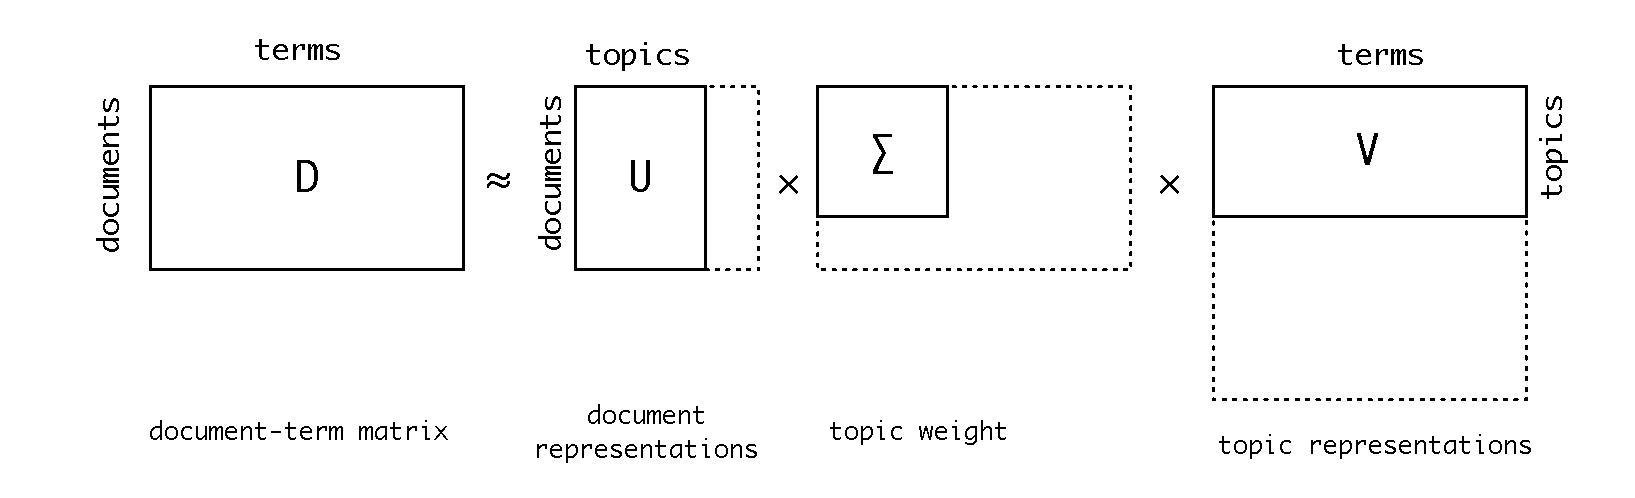
\includegraphics[width=1\textwidth]{fig/SVD.pdf}
    \caption{the sketch of the process of LSI using SVD}
    \label{fig:svd}
\end{figure}

The LSI model is able to recognize synonyms and reduce the adverse impact of noise of data, so that the documents are profiled more precisely and more stably.  However, it has also disadvantages. On the one hand, SVD is an operation with high complexity of runtime and memory. When a huge number of documents are trained or the model needs to update, the cost of SVD is probably intolerable (see section \ref{sec:5.3}). On the other hand, the meaning of the components of $V$ and $U$ cannot be interpreted as a kind of human understanding. 

\subsubsection{Latent Dirichlet Allocation}

LDA was presented as a probabilistic graphical model by \cite{Blei:2003}. LDA is a BoW-based topic model, which can compute the probability distribution of topics for a given document. Moreover, topics can be represented as a series of weighted words by LDA. 

The LDA model (\cite{Blei:2003}) is a Bayesian generative model. From the view point of LDA, a document is generated in the following phases:

\begin{itemize}
    \item[1.] select the topic distribution $\theta_i$ of the target document $d_i$ from the prior Dirichlet distribution $\alpha$, 
    \item[2.] generate a topic $z_{i,j}$ of $j$th word in the document $d_i$ from the multinomial topic distribution $\theta_i$ using Gibbs sampling,
    \item[3.] generate a word distribution $\Phi_{z_{i,j}}$ of the topic $z_{i,j}$ from the prior Dirichlet distribution $\beta$ using Gibbs sampling, 
    \item[4.] generate the word from the multinomial word distribution $\Phi_{z_{i,j}}$. 
\end{itemize}

The progress of generation is illustrated by figure \ref{fig:lda}.

\begin{figure}[!htb]
    \centering
    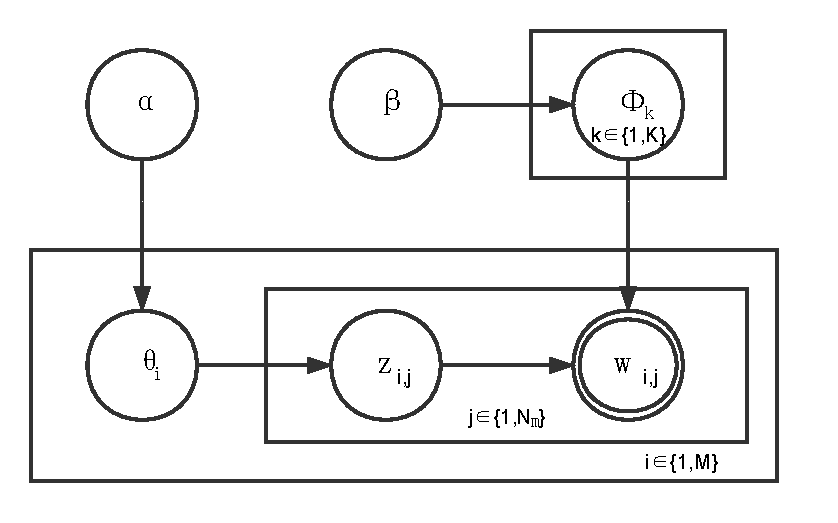
\includegraphics[width=0.5\textwidth]{fig/lda.pdf}
    \caption{Plate notation of representation of LDA. The dual-line plate refers to the observed variable, i.e. the posterior distribution of words in this case, and the monocoil plates indicate the latent variables, such as topic distribution and word distributions given a topic. The direction of arrows refer the conditional dependency of variables. }
    \label{fig:lda}
\end{figure}

The LDA model provides a general idea to build topic model. Since the work of \cite{Blei:2003}, subsequent research has explored many variant of LDA. There are four kinds of topic models so far, where are 1) unsupervised and non-hierarchical, 2) unsupervised and hierarchical, 3) supervised and non-hierarchical and 4) supervised and hierarchical. The research and model names are drawn in the table \ref{tab:lda} respectively.

\begin{table}[!htb]
\centering
\resizebox{\textwidth}{!}{%
\begin{tabular}{|l|l|l|}
\hline
\textbf{Topic Models} & \textbf{non-hierarchical} & \textbf{hierarchical} \\ \hline
\textbf{unsupervised} & \begin{tabular}[c]{@{}l@{}}LDA \cite{Blei:2003} \\ Correlated Topic Model \cite{blei2006correlated} \end{tabular} & HLDA \cite{sivic2008unsupervised} \\ \hline
\textbf{supervised} & \begin{tabular}[c]{@{}l@{}}sLDA \cite{Blei:2008wy} \\ labeled LDA \cite{ramage2009labeled} \end{tabular} & HSLDA \cite{perotte2011hierarchically} \\ \hline
\end{tabular}%
}
\caption{Topic Models Variant of LDA}
\label{tab:lda}
\end{table}

\subsection{Recommendation System}

\subsection{Research Question}

There is a nontrivial way from semantic text similarity to relatedness of documents. We attempt to find a systematic measure to discover related articles by given a target one. The main task is to discover 2\textasciitilde 5 candidate of related articles from a large corpora by given a target document. The most of researches have only discussed the degree of similarity between documents or the proportion of topics in each document and in the corpus. However, text similarity does not mean relatedness, neither do a few shared topics of documents. For example, a piece of news reporting the personal financial problems of the president Obama and another discussing making the financial policy of the president Obama are unrelated to each other by human understanding, whereas the STS measures treat them as related articles due to the high score of text similarity. More about this kind of errors will discuss in section \ref{5.5}. Four major questions have to be answered, so that achieving the relatedness degree of documents can be formulated more properly: 

\begin{itemize}
    \item[1.] \label{q:1}[1] Can Semantic Text Similarity including string-based and vector space models methods be used to find related articles? How effective and efficient is the metrics of performance, such as precision and operating time?
    \item[2.] \label{q:2}[2] Taking reducing time and memory usage into account, some documents, which are clearly unrelated to the target, should be filtered before processed by STS measures.  Can a filtering method based on data and meta-data be applied to reduce the number candidates that must be checked?
    \item[3.] \label{q:3}[3] Is it useful to combine STS methods with semantic vector space? Does it yield to an improvement in performance or to a significant decrease of runtime?
    \item[4.] \label{q:4}[4] The above introduced methods are unsupervised. Does it lead to an improvement when (semi-) supervised methods are utilized?
\end{itemize}
  \clearpage
  \section{Description of Dataset, Task and Evaluation}
\label{sec:3}

In this section we introduce the target dataset, the structure of articles and the relationship between articles which is regarded as a graph, called corpus-graph. Then, we bring forward the task of our work that a framework or a recommendation system is designed to discover related articles automatically instead of accomplishing the job manually. The final goals is to make the break-even point between the precision of predicting and the operating performance. In the end of the section, we discuss which evaluation methods are chosen and the reason thereof. 

\subsection{Description of Dataset}
\label{sec:3.1}

Our task concentrates on the corpus \textbf{ZEIT} ONLINE. ``DIE ZEIT'' (eng. ``the time'') is a German national weekly newspaper and ``ZEIT ONLINE''\footnote{ZEIT ONLINE: http://www.zeit.de/index} is the corresponding online representation. More than 300,000 articles, which are released between 1946 and 2014 and marked into 20 different categories, are collected in the corpus. Basically, one or two articles are indicated as recommended reading for each article. In the past, normally, this kind of assignments is completed by editors manually. The motivation of this research is to find an automatic or semiautomatic alternative approach to accomplish the job. Foremost, the elementary information and statistic are useful for a better understanding of the corpus. 

\subsubsection{Meta-data and Structure}
\label{sec:3structure}

The record of each article consists of a structure of meta-data, which describe the elementary information of the article. The structure is introduced briefly in this section. Then a typical example is depicted in figure~\ref{fig:article_structure}.



\begin{description}
    \item[URL] the hyperlink as the entry to access the article.

    \item[Title] a descriptive heading or caption, in which the article is summarized.
    \item[Supertitle] a label of the article, which indicates a particular theme under the category.
    \item[Summary] a couple of sentences where is used for arousing the interest of reader and which are the explaination of the background or the summarization of the article. 
    \item[Author] the writer of the article.
    \item[Release date] the timestamp of publishing the article. The distribution is illustrated in table \ref{tab:release_dist}.
    \item[Category] the category which the article belongs to. The distribution is illustrated in table \ref{tab:cate_dist}.

    \item[Content] the main body of the article.
    
    \item[Keywords] a couple of nouns or phrases which are significant for the article and can be used for retrieval. Normally, the vocabulary of all possible keywords is maintained manually. 
    
    \begin{figure}[!htb]
    \centering
    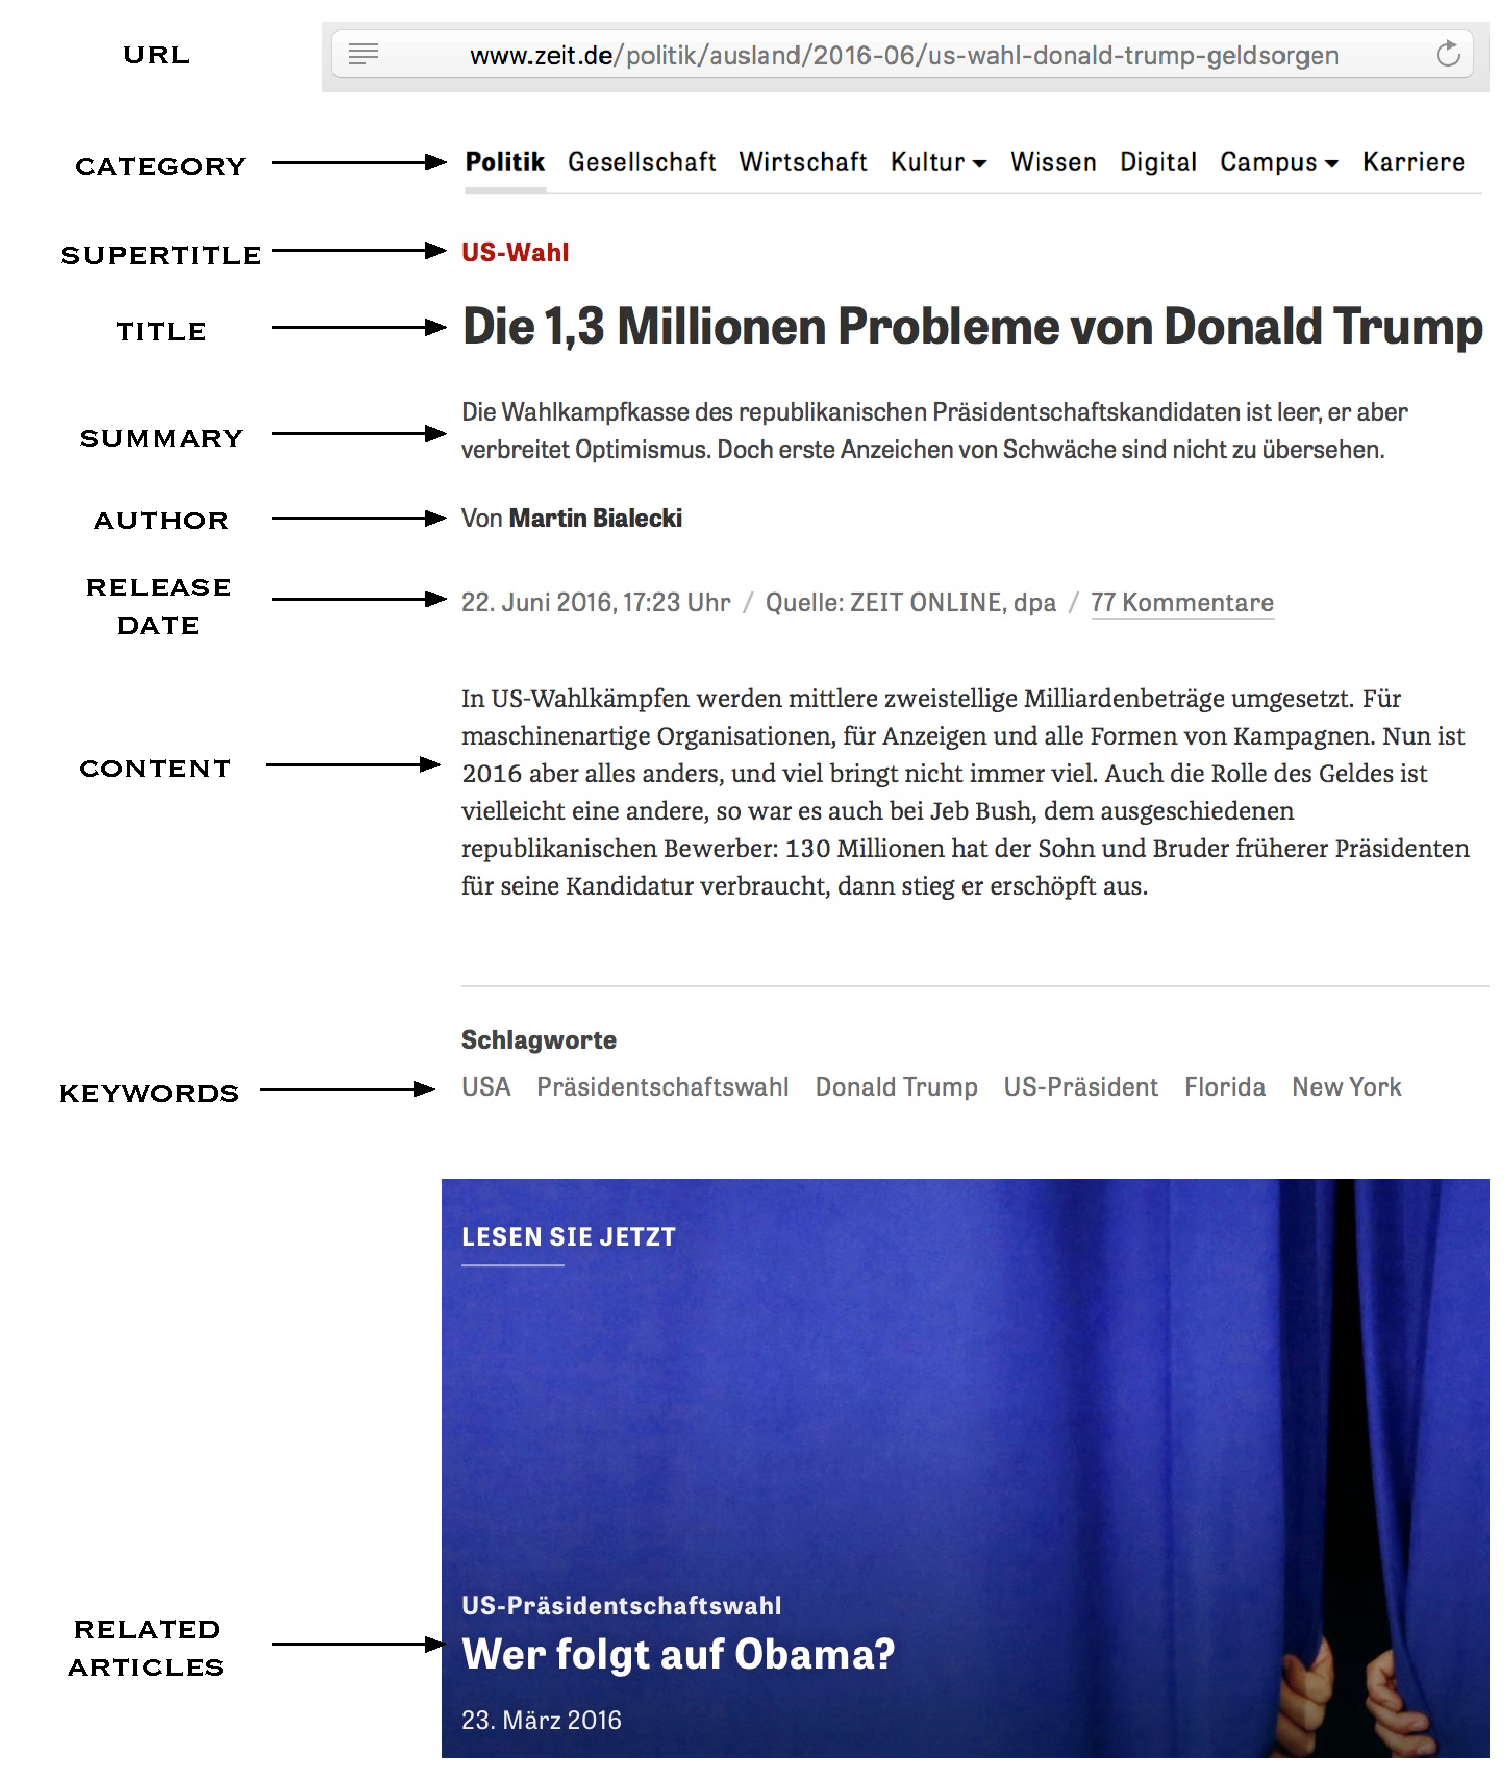
\includegraphics[width=1\textwidth]{fig/article.pdf}
    \caption{a typical example of the structure and meta-data of articles}
    \label{fig:article_structure}
    \end{figure}
    
    \item[Related articles] the recommendation for extended reading according to the current article. The related articles may have the same topic, similar background, or causal relationship to the current article.
    
        \begin{table}[!htb]
        \begin{minipage}{.45\linewidth}
        \centering
        \begin{tabular}{rrr}
        \hline
            \textbf{year} &   \textbf{quantity} &   \textbf{proportion (\%)} \\
        \hline
         1946 &     822 &             0.27 \\
         1947 &     658 &             0.22 \\
         1948 &    1715 &             0.56 \\
         1949 &    1579 &             0.52 \\
         1950 &     855 &             0.28 \\
         1951 &     662 &             0.22 \\
         1952 &     588 &             0.19 \\
         1953 &     612 &             0.20 \\
         1954 &     540 &             0.18 \\
         1955 &     794 &             0.26 \\
         1956 &     728 &             0.24 \\
         1957 &     660 &             0.22 \\
         1958 &     774 &             0.25 \\
         1959 &     737 &             0.24 \\
         1960 &    1613 &             0.53 \\
         1961 &    3517 &             1.15 \\
         1962 &    3408 &             1.12 \\
         1963 &    3517 &             1.15 \\
         1964 &    3984 &             1.31 \\
         1965 &    4405 &             1.44 \\
         1966 &    4851 &             1.59 \\
         1967 &    4662 &             1.53 \\
         1968 &    5068 &             1.66 \\
         1969 &    5299 &             1.74 \\
         1970 &    5293 &             1.73 \\
         1971 &    4596 &             1.51 \\
         1972 &    5266 &             1.73 \\
         1973 &    5155 &             1.69 \\
         1974 &    4596 &             1.51 \\
         1975 &    3804 &             1.25 \\
         1976 &    3616 &             1.18 \\
         1977 &    3535 &             1.16 \\
         1978 &    3606 &             1.18 \\
          1979 &    2969 &             0.97 \\
         1980 &    2964 &             0.97 \\
        \hline
        \end{tabular}
        \end{minipage}
        \begin{minipage}{.45\linewidth}
        \centering
        \begin{tabular}{rrr}
        \hline
            \textbf{year} &   \textbf{quantity} &   \textbf{proportion (\%)} \\
        \hline
         1981 &    3432 &             1.12 \\
         1982 &    2898 &             0.95 \\
         1983 &    2849 &             0.93 \\
         1984 &    2831 &             0.93 \\
         1985 &    4363 &             1.43 \\
         1986 &    4138 &             1.36 \\
         1987 &    4499 &             1.47 \\
         1988 &    4328 &             1.42 \\
         1989 &    4361 &             1.43 \\
         1990 &    4242 &             1.39 \\
         1991 &    4476 &             1.47 \\
         1992 &    4604 &             1.51 \\
         1993 &    4001 &             1.31 \\
         1994 &    4498 &             1.47 \\
         1995 &    5767 &             1.89 \\
         1996 &    5765 &             1.89 \\
         1997 &    5510 &             1.81 \\
         1998 &    2560 &             0.84 \\
         1999 &    5681 &             1.86 \\
         2000 &    6904 &             2.26 \\
         2001 &    7124 &             2.33 \\
         2002 &    4578 &             1.50 \\
         2003 &    4475 &             1.47 \\
         2004 &    5049 &             1.65 \\
         2005 &    5031 &             1.65 \\
         2006 &    2782 &             0.91 \\
         2007 &    1350 &             0.44 \\
         2008 &    6746 &             2.21 \\
         2009 &   14836 &             4.86 \\
         2010 &   15328 &             5.02 \\
         2011 &   14396 &             4.72 \\
         2012 &   15419 &             5.05 \\
         2013 &   16827 &             5.51 \\
         2014 &    6039 &             1.98 \\
         nan &     15    &            0.00 \\ 
        \hline
        \end{tabular}
        \end{minipage}
        \begin{minipage}{1\linewidth}
        \centering
        \begin{tabular}{rrr}
        \\
        \textbf{total} & 305222 & 100.00 \\
        \hline
        \end{tabular}
        \end{minipage}
        \caption{Release date distribution of the corpus}
        \label{tab:release_dist}
        \end{table}

        \begin{table}[!htb]
        \begin{minipage}{.45\linewidth}
        \centering
        \begin{tabular}{rrr}
        \hline
            \textbf{year} &   \textbf{quantity} &   \textbf{proportion (\%)} \\
        \hline
         Politik      &      80482 &            26.37 \\
         Wirtschaft   &      57530 &            18.85 \\
         Kultur       &      55794 &            18.28 \\
         Gesellschaft &      27600 &             9.04 \\
         Wissen       &      26078 &             8.54 \\
         Lebensart    &      23714 &             7.77 \\
         Reisen       &      13968 &             4.58 \\
         Sport        &       7427 &             2.43 \\
         Digital      &       4267 &             1.40 \\
         Karriere     &       3352 &             1.10 \\
        \hline
        \end{tabular}
        \end{minipage}
        \begin{minipage}{.45\linewidth}
        \centering
        \begin{tabular}{rrr}
        \hline
            \textbf{year} &   \textbf{quantity} &   \textbf{proportion (\%)} \\
        \hline
         Studium      &       2551 &             0.84 \\
         Literatur    &       1384 &             0.45 \\
         Deutschland  &        369 &             0.12 \\
         Hochschule   &        360 &             0.12 \\
         Auto         &        147 &             0.05 \\
         Musik        &         88 &             0.03 \\
         Gesundheit   &         53 &             0.02 \\
         Meinung      &         51 &             0.02 \\
         Kunst        &          6 &             0.00 \\
         Schule       &          1 &             0.00 \\
        \hline
        \end{tabular}
        \end{minipage}
        \begin{minipage}{1\linewidth}
        \centering
        \begin{tabular}{rrr}
        \\
        \textbf{total} &  305222 & 100.00 \\
        \hline
        \end{tabular}
        \end{minipage}
        \caption{Category distribution of the corpus}
        \label{tab:cate_dist}
        \end{table}
        
\end{description}

\subsubsection{Relatedness and Corpus-Graph}

As introduced in the previous section, each article has one or two recommended articles. From the viewpoint of graph theory, the corpus is treated as a undirected graph, in which articles are regarded as vertices and the relationship of recommendation are as edges between the target article and recommended articles. Formally, two articles can be labeled as ``related''-by-$h$ to each other, if a path between them exists in the path and the length thereof is shorted than the pre-defined value $h$ (by default: 3). For instance represented in figure \ref{fig:relatedness}, article $A$ is related to article $B, C, D, E, F, F, G$, and unrelated to  article $H$ (too far from the target), $I, J, K$ (unreachable from the target). 
 
\begin{figure}[!htb]
    \centering
    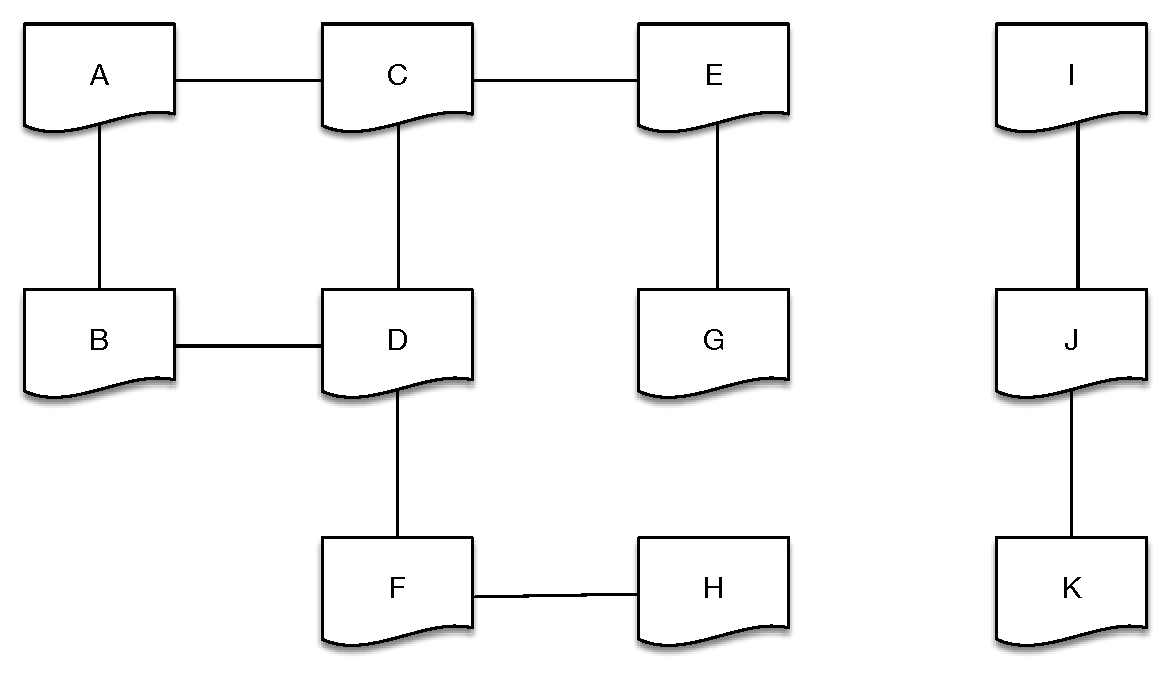
\includegraphics[width=0.75\textwidth]{fig/relatedness.pdf}
    \caption{a schematic graph of articles and relationship of relatedness}
    \label{fig:relatedness}
\end{figure}


\subsection{Description of Task}
\label{sec:3.2}

In the past, the relationship of relatedness are labeled typically by the author. However, this way has some disadvantages. On the one hand, the job need more human costs. On the other hand, the selection of candidates is limited by the work capacity and knowledge of the author, and these level is not stable. So it is necessary to exploit an automatic framework to discover related articles. The input of the framework is a article represented in a structure described in section~\ref{sec:3structure}, while the output is $k$ (in our case, $k=2$) articles which are marked as ``related'' normally with highest score or probability computed by the model. After determining the input and the expected output format, the main task is to train the model with the corpora of historical articles. The training methods are classified into unsupervised and supervised methods. The both kinds of methods are elaborated in section~\ref{sec:xxx}. In the scenario of reality, articles come in chronological order and the corpora which is as dataset of candidates has to be updated timely, because articles which are close to each other in time prefer to be more related than articles which are distant in time (see section \ref{sec:yyy}). Furthermore, it is also essential to update the model, in order to improve the precision, while operation of updating is costly and will lead to decrease the operating performance. Another task is, hence, to find an incremental method of updating and the trade-off between the effectiveness (precision) and efficiency (operating performance). The high-level depiction is drawn in figure~\ref{fig:highlevel}. 

\begin{figure}[!htb]
    \centering
    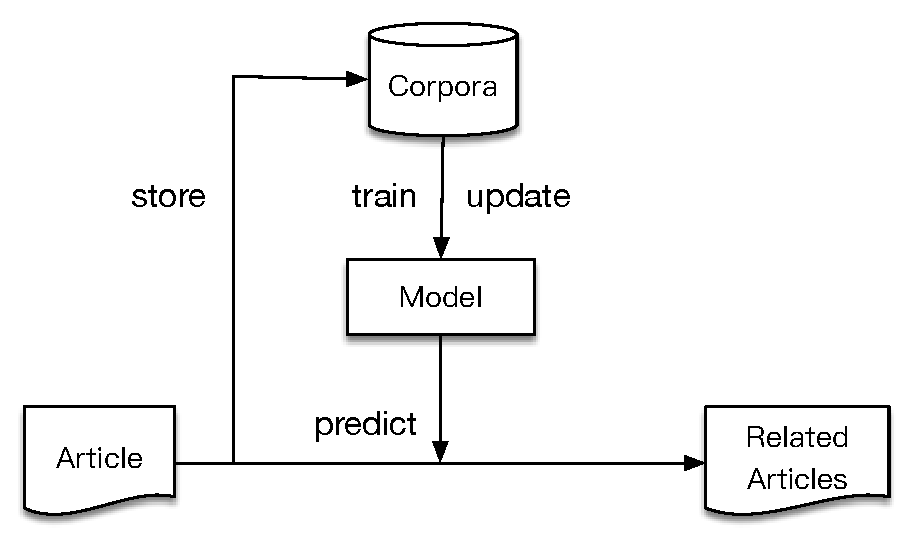
\includegraphics[width=0.6\textwidth]{fig/high-level.pdf}
    \caption{High-level depiction of the framework to discover related articles. }
    \label{fig:highlevel}
\end{figure}

\subsection{Evaluation Method}
\label{sec:3.3}

Effectiveness and efficiency are two main performance indicator. Effectiveness is about doing the right things. particularly in our case, it refers to whether the framework discovers related articles. Efficiency is about doing the things in optimal way, i.e., how much time and memory usage a series of operations to find related articles consumes. 

\subsubsection{Effectiveness}

The evaluation of effectiveness can be separated into two parts. One of them is to evaluate how well the final results and the other one is to indicate how well the entire ranking of candidates are computed by the framework given the target article. \textit{Precision@k@h} is used for the former and \textit{normalized Discounted Cumulative Gain} (\textit{nDCG}) is applied for the latter. 

\textit{Precision@k@h} is defined as the ratio of the number of the correct predictions to the number of predictions. Formally, given the corpora $D = \{d_1, d_2, \cdots, d_n\}$, a target set $T = \{t_1, t_2, \cdots, t_s\}$, the framework predicts $k$ related articles $P_i = \{d_{i_1}, \cdots, d_{i_k}\}$ for each article $i$ in $T$. Articles, which are at most $h$-hops apart from the target article, are regarded as the set $R_i^h$ of the true related articles of the article $i$ in $T$. 
\begin{equation}
    precision@k@h = \frac{\sum_{i=1}^s{|P_i \cap R_i^h|}}{k \cdot |T|}
\end{equation}

Unlike \textit{precision@k@h} which is applied to evaluate the final results of the framework, \textit{nDCG}, which is a measure of ranking quality in the field of information retrieval, focuses to evaluate the relatedness degree of the entire candidates. The framework makes a ranking of all $n$ candidates by the relatedness score or probability for a given target article $t$. Note that a article $d_i$ is placed at the position $i$ in the ranking. The relatedness degree is defined as $2^{-l}$ where $l$ is the distance between two articles in the corpus-graph.\footnote{$l=+\infty$ and the degree is $0$, if the articles are unreachable to each other.} We denote the degree between the target $t$ and a candidate $d_i$ by $ref_{d_i}^t$.

The formula to compute \textit{nDCG} of a target article $t$ is as followed. 

\begin{align}
   & nDCG_t = \frac{DCG_t}{IDCG_t} = (\sum_{i=1}^n\frac{ref_{d_i}^t-1}{log_2(i+1)})/(\sum_{i=1}^n\frac{ref_{d_i}^t-1}{log_2(r_{d_i}+1)})
\end{align}

Where $r_{d_i}$ is the position of $d_i$ of the ideal ranking which is generated by ordering by the relatedness degree. The \textit{nDCG} of the target set is $nDCG = \sum_{t \in T}nDCG_t$/s.

\subsubsection{Efficiency}

The newspaper is quite time-sensitive, so that it is significant that all tasks inclusive of discovery related articles should be completed as soon as possible. The time and memory usage of building model, predicting and updating model should be evaluated respectively. We focus mainly on the divergence between different methods in order to compare their relative merits, whereas the concrete value of time cost and memory usage depends on the performance of hardware and hence we discuss just whether the cost is in a reasonable range. For instance, the operation of predicting should be finshed in one minute maximal and it is reasonable and tolerable that building model is completed in one day or even a couple days. 
  \clearpage
  \section{Experimental Setup}
\label{sec:4}
In this section, we discuss how to design the framework for discovering related articles in the corpus. As described in section \ref{sec:3}, each article contains semantic data including title, summary and content, together with meta-data, which consists of category, keywords, release date and the number of words in the texts. The purpose of this section is to evaluate how the methods which are mentioned in section \ref{sec:2} work in effectiveness and efficiency together with different semantic data. Then the assessment of filtering method which reduces the number of candidates with combining the meta-data is analyzed. In other words, this section focuses on finding the answer of question 1 and 2.

In section \ref{sec:4.1} the theoretical feasibility and challenge is discussed. The definition of terms and notations which are used in the rest sections is brought forwards in section \ref{sec:4.2}. In section \ref{sec:4.3} we discuss the design of experiments according to the application scenarios and depict the architecture of the framework. Furthermore, the setup of experiments is described in section \ref{sec:4.4}, including the setup of dataset given to experimenting and the setup of alternative models. 

\subsection{Theoretical Feasibility and Challenge}
\label{sec:4.1}

All STS methods and VSM models which are introduced in section \ref{sec:2}, are usually applied for computing the semantic similarity between texts. However, our goal is to find related articles for given target articles. Foremost, the difference between the term \textit{similarity} and \textit{relatedness} must be understood. The terms \textit{similarity} and \textit{relatedness} are two separate concepts\cite{pedersen2007measures}. \textit{Similarity} is the measure which indicates how a text looks like another text semantically, while relatedness is a more general concept, which contain multiple notions, such as causal relationship, temporal relationship and the relationship shared the identical event or background. We illustrate the difference with two examples. 

\begin{description}
\item[Example 1] There are two pieces of news. One of them reports the football game of Euro Champions between FC Bayern and Real Madrid in 2014, while the other reports the football game of German Bundesliga between FC Bayern and Dortmund in 2015. Obviously, they are similar to each other semantically, because they share the same topic (football game) and the same subject (FC Bayern).Meanwhile, they are unrelated to each other. The reason is that the two games are held in the different seasons and the different competitions. Exactly, football games is quiet a kind of short-term and event-sensitive events. 
\item[Example 2] Case TBD. They are not similar, because they may share quieta few words and meaning. However, they are related, because the both are about the consequence of TBD. The prediction of relatedness requires knowledge of the background in this case.
\end{description}

From the two examples, we can draw a conclusion, that computing relatedness is much more complicated than computing similarity, because the machine must understand exactly how humankind understands the identities and the differences between two articles as well as the significant degree thereof. However, \textit{similar} documents and \textit{related} documents have a non-negligible intersection normally. Our task is derived from a scenario of reality that two related articles need to be assigned for every current article. Therefore, it is unnecessary to find all possible related articles but it is acceptable to find only a subset of them. From this goal, a way from computing \textit{similarity} to getting \textit{related} articles is feasible. 

Certainly, discovery related articles using similarity methods leads to bias. It means, that the framework prefers predicting related articles only with specific characteristics and consequently some articles will never be assigned, e.g. articles which have the identical background with the target. The bias and error analysis are discussed in section \ref{sec:5}.

\subsection{Definition and Notions}
\label{sec:4.2}

In the following sections, a series of concepts is mentioned frequently. In order to avoid ambiguity and misapprehension, the definition and interpretation of these terms are given in the following table.

\begin{description}[1cm]
\item[article] an instance of a piece of news or report, which contains the complete information or rather texts of title, summary and content as well as meta-data 
\item[document] a specific component of an article; any of title, summary or content in string format; refers to the text of content without any explicit declaration 
\item[candidate] all articles of the historic corpus,  
\item[term]  
\item[token]

\label{tab:def_terms}
\end{description}



\subsection{Architecture of Framework and Experiments Design}
\label{sec:4.3}

The high-level architecture of the framework was already depicted in figure \ref{fig:highlevel}. In this section, we explain how the framework predicts related articles and improves itself. 

The framework consists of four phases of preprocessing, model building, similarity computing and model updating. The architecture of the framework is illustrated in figure \ref{fig:unsupervised}. 

\begin{figure}[!htb]
    \centering
    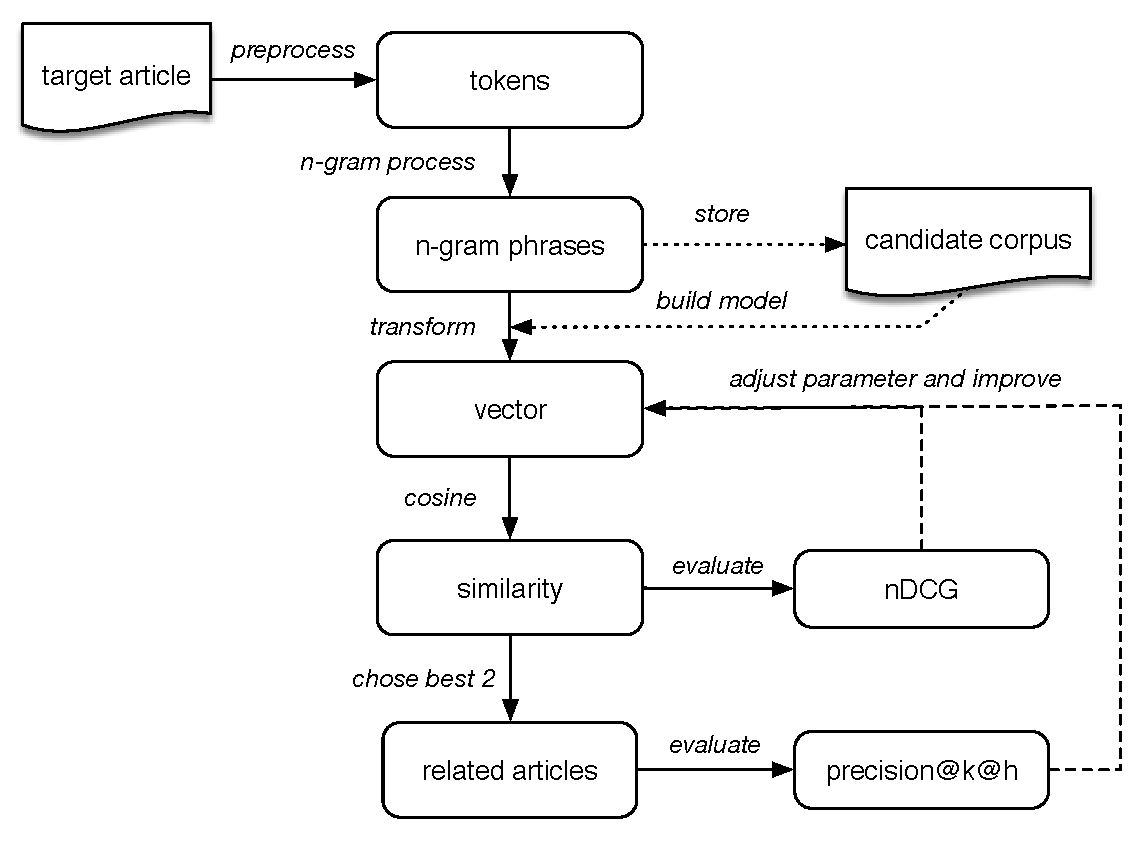
\includegraphics[width=0.7\textwidth]{fig/unsupervise}
    \caption{The architecture of the framework to discover related articles.}
    \label{fig:unsupervised}
\end{figure}


\subsubsection{Preprocessing}
The original data of title, summary and content is stored in the strings in HTML format. After all markups are removed and all characters are converted to small case, preprocessing separates the strings into the respective sequences of tokens. Four common methods are explained as follows:

\begin{description}
\item[\underline{SP}lit] The string is splitted into a sequence of tokens with the special characters (whitespace, hyphen and punctuations). 
\item[\underline{S}t\underline{E}m] Tokens, which are the result from the method \textit{SP} are replaced by the respective stems. For example, ``book'' is the stem of ``books'', ``booking'' and ``booked''. The advantage of stemming is to reduce the vocabulary size and decrease computational complexity and avoid overfitting of building semantic models. However, stemming causes the more serious problem of polysemy. 
\item[\underline{ST}op] After \textit{SP}, the stopwords, which are the most common words in a language, such as pronouns and prepositions are filtered out from the sequence. 
\item[\underline{S}tem+\underline{S}top] The data is handled by both of \textit{SP} and \textit{SE}. 
\end{description}

Preprocessing contains a sub-component, called n-gram processing. In our case, unigram, bigram and trigram are applied. In total, we have $4 \times 3 = 12$ alternative preprocessing methods. After preprocessing, the strings are represented as the respective sequences which the semantic models are able to deal with directly. 

\subsubsection{Model Building and Similarity Computing}
The component of model building is meaningful exclusive for VSMs. The approaches are quite different according to different models.  The detailed methods are described in the following list respectively.

\begin{description}
\item[BoW] BoW is the simplest and most basic model in VSMs. Each document is represented as a vector in which the weight of each dimension is the occurrence frequency of the respective term. In order to reduce the dimension of vectors, the terms which occur in the corpus at least $k$ times (in our case $k=5$) remain in the vocabulary. The BoW vector of a given document is independent of the rest corpus, so long as the vocabulary is constant. 
\item[tfidf] Tfidf is the model based on BoW, but the vector is relevant to the corpus. The tool to build tfidf model and the following models is \textit{gensim}\footnote{gensim is a NLP tool, which focuses on topic modeling and retrieving semantically similar documents \cite{rehurek_lrec}. Offical website:  https://radimrehurek.com/gensim/}.
\item[LSI and LDA] We build the models LSI and LDA based on tfidf. Both models are capable to reduce the dimension of vectors from the vocabulary size to the number of topics. It is therefore necessary to determine the optimal number of topics, in order to make balance between the precision and computational performance. 
\end{description}

In VSMs, each document is transformed as a vector and the semantic similarity to other documents is the \textit{cosine} similarity between the vector of the target document and the vector of candidate documents. The articles in the historic corpus which are the most \textbf{two} similar to the given target article are predicted as the related articles. 

\subsubsection{Model Updating}

In the application scenario of reality, once the related articles are selected for a given article, the recent article should be stored in the historic corpus as the candidate articles for future articles. The characteristics (e.g. topic distribution, new popular words) of the corpus is rearranged over time. Therefore the models need updating incrementally, in order to be able to reflect the attributes of the corpus in time. However, it is costly for computational time and power to update models. In our case, it is also one research task, to find trade-off between delay of updating and cost of time.

\subsection{Experiment Description}
\label{sec:4.4}

1. 选择最好的pp+model 
2. 随着文章的增加,对性能的影响

\subsection{Dataset}

The elementary structure and information is described in section \ref{sec:3.1}. Now we generate the dataset as the input of the framework. Articles, which have no related articles or no \textit{title}, or whose content is less than 1000 characters, are filtered. Furthermore, articles which belong to a weak category \footnote{Weak category: the amount of articles in this category is fewer than $1\%$ of the corpus size} or which were released before 2009 are removed from the corpus. We have $75908$ articles in $7$ categories. The category distribution is drawn in table \ref{tab:cate_dist_new} and the release date distribution is in table \ref{tab:release_dist_new}

\begin{table}[!htb]
\centering
\begin{tabular}{lrr}
\hline
\textbf{category} &   \textbf{quantity} &   \textbf{proportion (\%)} \\
\hline
Politik      &      26071 &            34.35 \\
Wirtschaft   &      12531 &            16.51 \\
Kultur       &       8584 &            11.31 \\
Gesellschaft &       7646 &            10.07 \\
Wissen       &       5273 &             6.95 \\
Sport        &       4993 &             6.58 \\
Digital      &       3887 &             5.12 \\
Reisen       &       2199 &             2.90 \\
Karriere     &       2169 &             2.86 \\
Studium      &       1570 &             2.07 \\
Lebensart    &        985 &             1.30 \\
\hline
\textbf{total}        &      75908 &           100.00 \\
\hline
\end{tabular}
\caption{Category distribution of \textit{ZEIT} corpus after filtering unsatisfied articles}
\label{tab:cate_dist_new}
\end{table}
\begin{table}[!htb]
\centering
\begin{tabular}{rrr}
\hline
\textbf{year} &   \textbf{quantity} &   \textbf{proportion (\%)} \\
\hline
2009 & 12628 &            16.64 \\
2010 & 14716 &            19.39 \\
2011 & 13970 &            18.40 \\
2012 & 14583 &            19.21 \\
2013 & 14941 &            19.68 \\
2014 &  5070 &             6.68 \\
\hline
\textbf{total} & 75908 &           100.00 \\
\hline
\end{tabular}
\caption{Release date distribution of \textit{ZEIT} corpus after filtering unsatisfied articles}
\label{tab:release_dist_new}
\end{table}

\begin{description}
\item[Experiment 1] $2000$ articles are selected randomly from the corpus as the test dataset, and the others are as the history data which is utilized to build unsupervised models. After that, the scores of relatedness of the tested articles are as the training dataset of supervised models. The supervised models will be trained by these data in the cross-validation way. 
\item[Experiment 2] The articles in corpus are sorted by the \textit{release date}, so that the real-world scenario can be simulated. The articles, which were published before 2013, are as the training data to initialize unsupervised models. There are two phases to deal with each target article, that are predicting related articles from the historical corpus and updating the model incrementally. Then the supervised methods make use of the scores from the unsupervised methods to compute the integrated scores and discover the related articles for each target article. 
\end{description}

\subsection{Features}

\subsubsection{Meta-data}

\subsubsection{Semantic Features}

\subsection{Supervised Methods}



  \clearpage
  %!TEX root = <../index.tex>

\section{Experimental Results and Discussion}
\label{sec:5}

The experimental results are described, analyzed and concluded in this section. In section \ref{sec:5.1} the statistics of the corpus after preprocessing is showed briefly. Section \ref{sec:5.2} focuses on the effectiveness of the different STS models, i.e. how precisely the STS models judge an articles as related for a given target article. Furthermore, the operational performance of the STS models is reported in section \ref{sec:5.3}. The above three parts concentrate on the results of the first experiment, which is mentioned in section \ref{sec:4.4}. On the next step, the results of the second experiment are reported in section \ref{sec:5.4}. After reporting the results of the both experiments, we discuss the most severe types of errors that an articles which is virtually unrelated is judged as related for a target article or a cluster of articles which are properly related are never or rarely judged as related. In conclusion, we summarize the consequence of selection of the STS models and the challenge of the current work. 

\subsection{Analysis of Preprocessing}
\label{sec:5.1}

Each article contains three semantic components, so-called text sources, including \icontent{}, \ititle{}, \isummary{} which are as input data of the framework. After preprocessing the text sources in raw string format is converted to a sequence of words which consist of $n$ tokens. 

\begin{figure}[!htb]
    \centering
    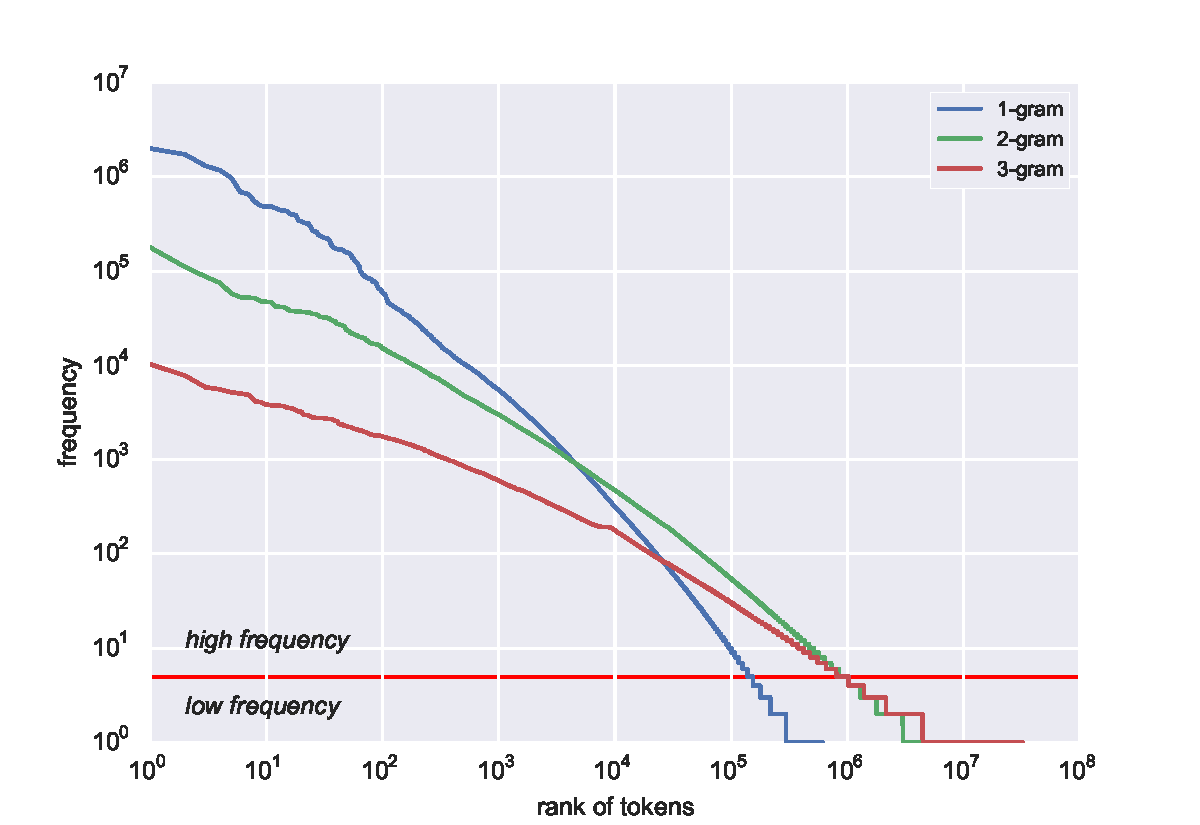
\includegraphics[width=0.8\textwidth]{fig/freqdist}
    \caption{Occurrence Frequency of terms in the corpus for uni-, bi- and trigram in descend ranking. The corresponding preprocessing is \iSE{} and the text source is \icontent{}.}
    \label{fig:freqdist}
\end{figure}

There are two attributes to portray a vocabulary. The first attribute is the size, which decides the computation complexity, such as the dimension of vector space. The second one is the scale of ``long tail'' of the vocabulary. The ``long tail'' is the part of the distribution which contains a large number of elements with low occurrence frequency. In our case, the threshold of ``long tail'' is $5$, in other words, the terms occurring less than $5$ times belong to the ``long tail'' of the vocabulary. According to the Zipf's law, the occurrence frequency is distributed extremely unevenly or that is to say that the most terms are rarely in use and hence it is almost incapable of determining the semantic relevance of these terms by statistical methods. In ideal case, a vocabulary with smaller size and fewer low-frequency terms has the better quality of operational complexity and semantic completeness. Figure \ref{fig:freqdist}, which depicts the representative distribution of the occurrence frequency of terms, indicates that only a small quantity of tokens occur repetitively in the corpus (25\% for unigram, 10\% for bigram and 3\% for trigram). In respect of efficiency, the tokens which appear less than $5$ times can be removed from the vocabulary. We denote the original vocabularies as \ifull{} vocabularies and the reduced vocabularies as \icommon{} vocabularies. 

We consider the size of \ifull{} vocabularies and the proportion of frequent tokens as the metrics to evaluate the vocabulary quality. Figure \ref{fig:vocab_size} shows the comparison between the size of \ifull{} and \icommon{} vocabularies which are generated by the preprocessing methods including \iSP{}, \iSE{}, \iST{} and \iSS{} in the different n-gram models ($n=1, 2, 3$) of the three types of text source containing \icontent{}, \ititle{} and \isummary{}. In the unigram model, \iSS{} always generates the vocabularies with the smallest size and the largest proportion of frequent terms as well. In bi- and trigram, the vocabularies generated by \iSE{} have the largest proportion of frequent terms and the size is slightly different with the vocabularies generated by other methods. In conclusion, the preprocessing method \iSS{} is applied in unigram and \iSE{} is applied in both of bigram and trigram in the application. 

\begin{figure}[!htb]
    \centering
    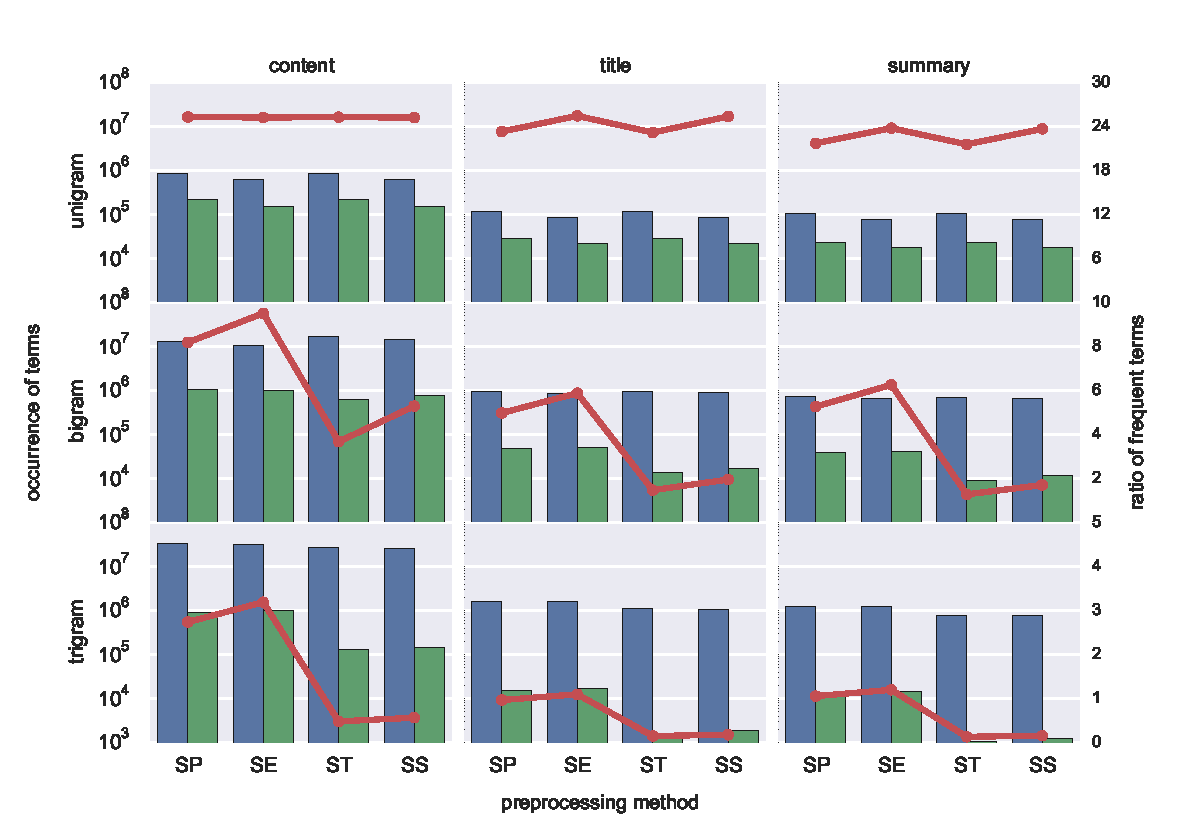
\includegraphics[width=\textwidth]{fig/vocab_size}
    \caption{Compare the vocabulary size of different NGF. \\ \begin{tabular}{ll} Column & types of text fields; \icontent{}, \ititle{} and \isummary{}, respectively \\ Row & corresponding n-gram models; uni-, bi-, trigram, respectively \\ Blue bars & \ifull{} vocabularies, \\ Green bars & \icommon{} vocabularies \\ Red lines & the ratio of the size of \icommon{} vocabularies to the size of corresponding \\ \ifull{} vocabularies.\end{tabular}}
    \label{fig:vocab_size}
\end{figure}


\subsection{Effectiveness of STS Models}
\label{sec:5.2}

As described in section \ref{sec:3.3}, the effectiveness metrics refer to \textit{precision@k@h} to evaluate the relatedness of the articles of top ranking and \textit{nDCG} to evaluate the overall results. First, the results for each preprocessed dataset are given and the best STS models is selected respectively. We give in advance the reasonable assumption that an article is true related to the articles which are not further than $3$ hops in the related-graph. Later in this part, the divergence between different categories is discussed and which categories the framework is more suitable for are concluded.  

\subsubsection{Parameter Selection for Topic Models}

Topic models, such as LSI and LDA, represent documents as vectors in the topic space. The dimension of the topic space, as well as the number of topics is pre-defined. Hence, it is necessary to determine the optimal number of topics before building and evaluating models. Figure \ref{fig:precision_topics} shows the change curve of precision and operational time of LSI with increasing the number of topics from $50$ to $1000$. The precision keeps increasing but the growth always becomes weaker, when the number of topics becomes larger. On the other side, the time cost of both of building and predicting increases with a relative stable growth speed. Out of the time limitation of the experiments, we select $500$ as the final value of this hyperparameter. The reason is the precision increases quite insignificantly with more than $500$ topics and we expect that the building time is limited to less than one hour and the predicting time is limited to less than one second. 

\begin{figure}[!htb]
    \centering
    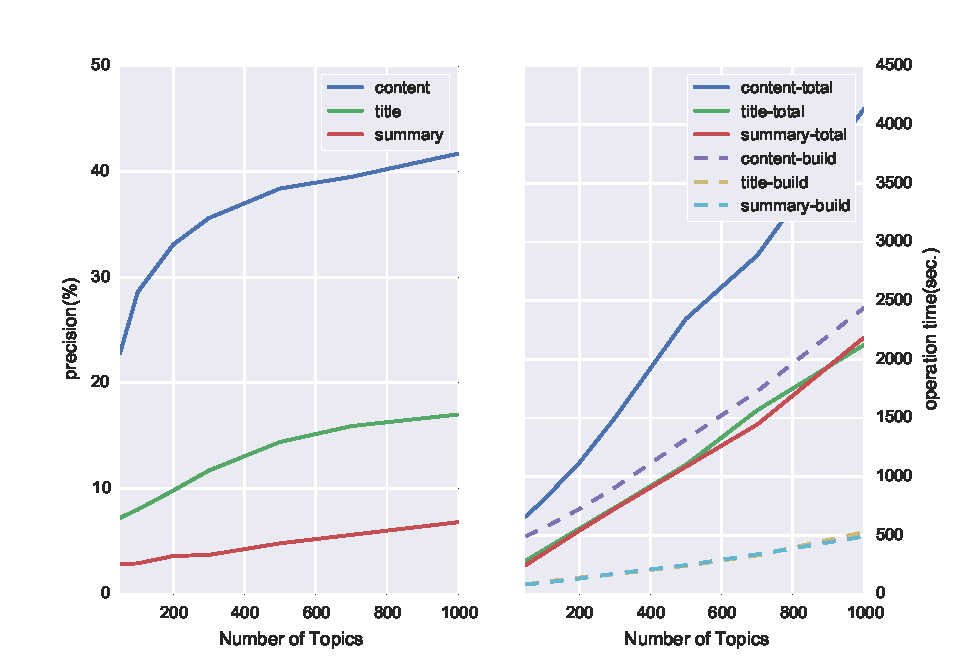
\includegraphics[width=\textwidth]{fig/precision_topics}
    \caption{Precision@2@3 and the time cost of LSI with the different value of the number of topics. Models are built with the historical corpus of $73908$ articles and predict related articles for $2000$ randomly selected articles. The dash line indicates the building time and the solid line indicates the total time including building and predicting. }
    \label{fig:precision_topics}
\end{figure}


\subsubsection{Overall Analysis of Effectiveness}

Figure \ref{fig:precision_2_3} compares the precision of the STS models in the different PDS. In general, the models perform in \icontent{} better than in \ititle{} and much better than in \isummary{}. Second, the precision in unigram is better than in bigram and the precision in trigram is the worst. To be specific, \textit{tfidf} preforms the highest precision for all data sources in unigram and for \icontent{} and \ititle{} in bigram. In the meanwhile, \textit{Jaccard} is stronger than the other models for \isummary{} in bigram and all data sources in trigram. \textit{LDA} is the weakest model all the time in the experiment and it is skipped in bigram and trigram to avoid unnecessary costs. The precision of \textit{BoW} is slightly ($10\% \sim 30\%$) lower than the best model and, however, it is $30\% \sim 60\%$ lower than the best model in bigram and trigram. 


\begin{figure}[!htb]
    \centering
    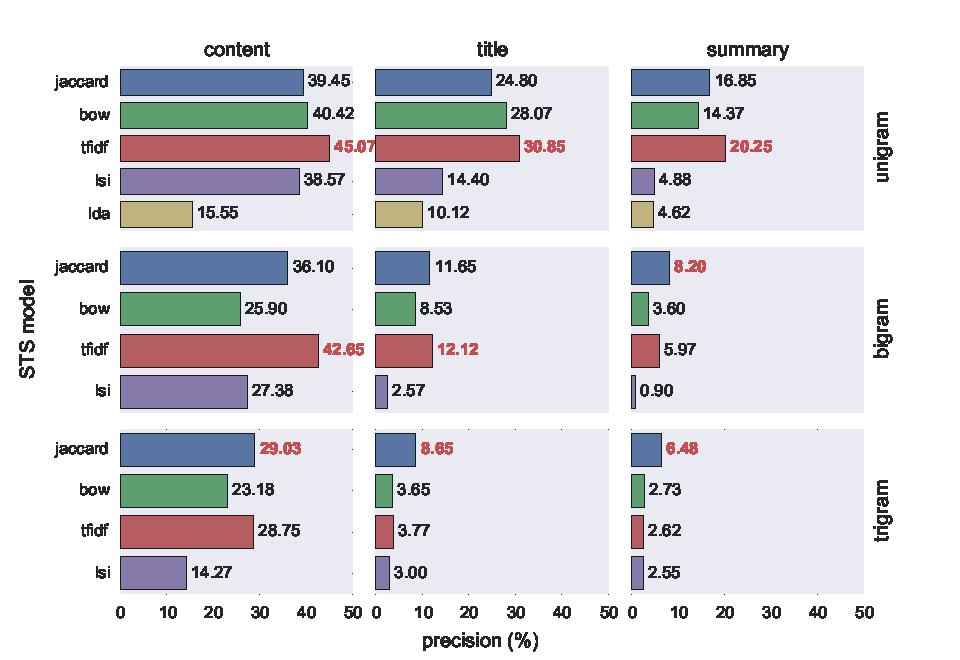
\includegraphics[width=\textwidth]{fig/precision_2_3}
    \caption{comparison the precision of \textit{jaccard}, \textit{BoW}, \textit{tfidf}, \textit{LSI} and \textit{LDA} for all data sources  with n-gram models. }
    \label{fig:precision_2_3}
\end{figure}

Figure \ref{fig:ndcg} illustrates the \textit{nDCG}, which is applied as the supplementary evaluation method. The order of models by \textit{nDCG} is similar to the results of \textit{precision} in general. All STS models are capable to discover related articles, because the measure \textit{nDCG} of every model is better than the baseline, which is computed for the random order of candidates. Moreover, LSI performs better in the metric \textit{nDCG} than in the metric \textit{precision} for the data source \icontent{}. To be specific, LSI is almost always at the second position after tfidf in \textit{nDCG}, whereas LSI is at the third or the last position in \textit{precision}. Accordingly, LSI computes the more precise relatedness of the overall corpus than jaccard and BoW, while LSI is not able to determine precisely which articles have the highest relatedness. 


\begin{figure}[!htb]
    \centering
    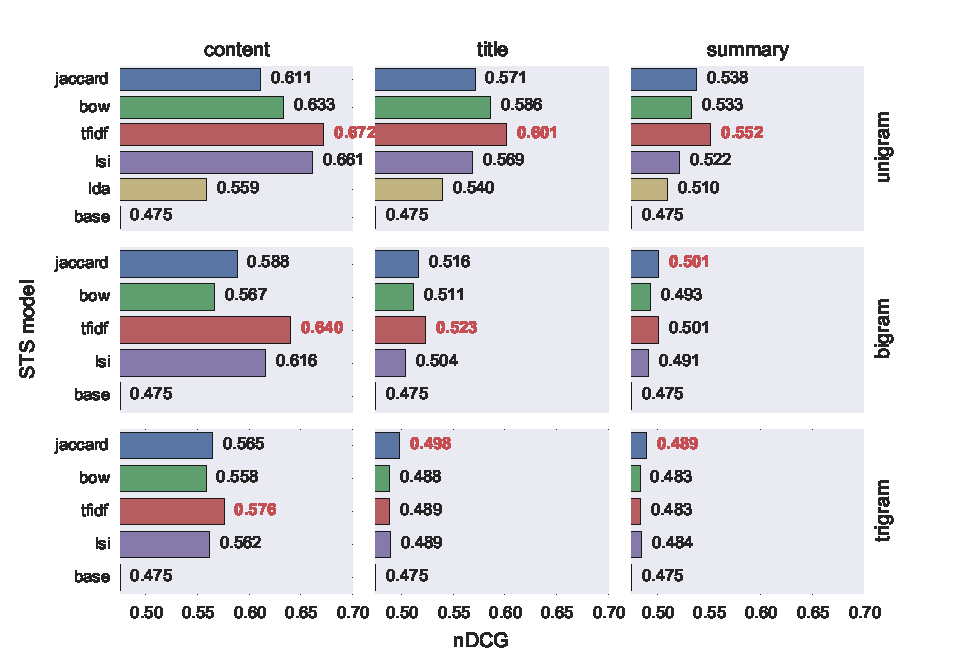
\includegraphics[width=\textwidth]{fig/ndcg}
    \caption{comparison the nDCG of jaccard, BoW, tfidf, LSI and LDA for all data sources with n-gram models.}
    \label{fig:ndcg}
\end{figure}


Combining the results of two evaluation methods, we conclude as follows.

1. Relatedness generated from data source \ititle{} or \isummary{} is worse than from \icontent{}, because \ititle{} and \isummary{} are short documents and then contain incomplete information. 

2. In n-gram, the vocabulary becomes larger and the relevance between phrases become weaker along with a greater $n$. On the other hand, a higher $n$ leads to the more serious loss of semantic information with removing the low frequency terms from the vocabulary. A typical example is that $77\%$ information/phrases are dropped through reducing vocabulary for \icontent{} in trigram. 

3. Tfidf is in the dominant position for uni-/bigram and long documents and jaccard is more suitable in trigram and short documents. Unexpected, LDA works with unsatisfactory effectiveness. 


%\subsubsection{Coverage of Related Articles Prediction}

\begin{table}[!htb]
\centering
\resizebox{\textwidth}{!}{%
\begin{tabular}{lrr|rr|rr|rr|rr|rr|rr|rr|rr}
 & \multicolumn{6}{c|}{\textbf{Content}} & \multicolumn{6}{c|}{\textbf{Title}} & \multicolumn{6}{c}{\textbf{Summary}} \\
 & \multicolumn{2}{c|}{\textbf{1-tfidf}} & \multicolumn{2}{c|}{\textbf{2-tfidf}} & \multicolumn{2}{c|}{\textbf{3-jaccard}} & \multicolumn{2}{c|}{\textbf{1-tfidf}} & \multicolumn{2}{c|}{\textbf{2-tfidf}} & \multicolumn{2}{c|}{\textbf{3-jaccard}} & \multicolumn{2}{c|}{\textbf{1-tfidf}} & \multicolumn{2}{c|}{\textbf{2-jaccard}} & \multicolumn{2}{c}{\textbf{3-jaccard}} \\
 & \multicolumn{1}{c}{\textbf{r}} & \multicolumn{1}{c|}{\textbf{diff}} & \multicolumn{1}{c}{\textbf{r}} & \multicolumn{1}{c|}{\textbf{diff}} & \multicolumn{1}{c}{\textbf{r}} & \multicolumn{1}{c|}{\textbf{diff}} & \multicolumn{1}{c}{\textbf{r}} & \multicolumn{1}{c|}{\textbf{diff}} & \multicolumn{1}{c}{\textbf{r}} & \multicolumn{1}{c|}{\textbf{diff}} & \multicolumn{1}{c}{\textbf{r}} & \multicolumn{1}{c|}{\textbf{diff}} & \multicolumn{1}{c}{\textbf{r}} & \multicolumn{1}{c|}{\textbf{diff}} & \multicolumn{1}{c}{\textbf{r}} & \multicolumn{1}{c|}{\textbf{diff}} & \multicolumn{1}{c}{\textbf{r}} & \multicolumn{1}{c}{\textbf{diff}} \\ \hline
\textbf{Mean} & \multicolumn{2}{c|}{45.07} & \multicolumn{2}{c|}{42.65} & \multicolumn{2}{c|}{29.03} & \multicolumn{2}{c|}{30.85} & \multicolumn{2}{c|}{12.12} & \multicolumn{2}{c|}{8.65} & \multicolumn{2}{c|}{20.25} & \multicolumn{2}{c|}{8.20} & \multicolumn{2}{c}{6.48} \\ \hline
\textbf{\textcolor{blue}{Gesellschaft}} & 3 & $+~~8.75$ & 4 & $+~~6.89$ & 2 & $+17.38$ & 3 & $+15.20$ & 4 & $+13.20$ & 2 & $+53.01$ & 2 & $+14.98$ & 2 & $+28.53$ & 2 & $+43.84$ \\
\textbf{\textcolor{blue}{Politik}} & 4 & $+~~8.24$ & 1 & $+14.57$ & 1 & $+41.88$ & 4 & $+~~6.97$ & 6 & $+~~5.00$ & 5 & $+~~6.89$ & 1 & $+16.26$ & 3 & $+16.23$ & 3 & $+10.94$ \\
\textbf{Digital} & 1 & $+15.83$ & 2 & $+~~9.97$ & 7 & $-34.45$ & 1 & $+24.78$ & 5 & $+13.13$ & 7 & $-23.27$ & 3 & $+~~9.25$ & 6 & $-19.06$ & 8 & $-31.66$ \\
\textbf{Kultur} & 6 & $-~~5.28$ & 6 & $-~~9.53$ & 9 & $-52.02$ & 6 & $-~~3.05$ & 1 & $+44.99$ & 4 & $+~~8.22$ & 4 & $+~~3.73$ & 4 & $+14.16$ & 5 & $+~~5.78$ \\
\textbf{Lebensart} & 10 & $-34.97$ & 10 & $-35.32$ & 6 & $-28.72$ & 9 & $-27.35$ & 2 & $+42.20$ & 1 & $+59.46$ & 9 & $-31.89$ & 1 & $+47.18$ & 1 & $+59.77$ \\
\textbf{Sport} & 7 & $-~~7.26$ & 5 & $-~~8.71$ & 5 & $-18.10$ & 7 & $-16.31$ & 3 & $+35.20$ & 8 & $-24.19$ & 5 & $-~~8.93$ & 5 & $-~~5.04$ & 6 & $-~~5.06$ \\
\textbf{Wissen} & 2 & $+13.10$ & 3 & $+~~8.04$ & 4 & $-17.81$ & 2 & $+15.46$ & 9 & $-38.01$ & 9 & $-24.44$ & 7 & $-14.47$ & 9 & $-32.25$ & 10 & $-44.48$ \\
\textbf{Karriere} & 5 & $+~~6.58$ & 7 & $-12.65$ & 8 & $-42.58$ & 5 & $-~~1.48$ & 10 & $-43.40$ & 6 & $-20.66$ & 6 & $-12.85$ & 8 & $-28.26$ & 4 & $+~~5.99$ \\
\textbf{\textcolor{red}{Wirtschaft}} & 8 & $-14.73$ & 8 & $-17.52$ & 3 & $-13.03$ & 8 & $-19.23$ & 8 & $-36.87$ & 10 & $-26.57$ & 8 & $-15.55$ & 7 & $-20.55$ & 7 & $-11.96$ \\
\textbf{\textcolor{red}{Reisen}} & 9 & $-30.22$ & 9 & $-31.93$ & 10 & $-52.77$ & 10 & $-34.65$ & 7 & $-20.19$ & 3 & $+11.88$ & 10 & $-64.16$ & 10 & $-50.83$ & 9 & $-37.73$ \\
\textbf{\textcolor{red}{Studium}} & 11 & $-61.03$ & 11 & $-49.30$ & 11 & $-67.41$ & 11 & $-43.05$ & 11 & $-66.56$ & 11 & $-37.51$ & 11 & $-73.31$ & 11 & $-83.52$ & 11 & $-79.13$ \\ \hline
\end{tabular}%
}
\caption{Comparison between the precision of different categories and the mean precision of the entire corpus. \textbf{r} refers to the ranking of precision in all categories and \textbf{diff} indicates the ratio (\%) of difference compared with the mean precision ($diff = \frac{prec_{cate} - prec_{mean}}{prec_{mean}}\times 100\%$)}
\label{tab:cate_precision}
\end{table}

\subsubsection{Divergence between Categories}

The effectiveness is reported and analyzed above in general. Now we are also interested, how the models, which are selected as the best models for each data set respectively, work for specific categories. The results are drawn in table \ref{tab:cate_precision}, where the precision ranking of each category and the difference ratio to the mean precision of the entire corpus are revealed. \textit{Gesellschaft} (\textit{society}) and \textit{Politik} (\textit{politics}) surpass the mean precision in all data set. On the contrary, \textit{Wirtschaft} (\textit{economics}), \textit{Reisen} (\textit{traval}) and \textit{Studium} (\textit{study}) are the worst performed categories. The precision of these three categories is much lower than the mean level. Taking content-unigram as example, the precision of the best category (\textit{Digital}) is about three times greater than the precision of the weakest category (\textit{Studium}). The results of predicting hence have  different confidence according to the category which the target article belongs to. Once the confidence of particular categories is lower than the threshold, the framework is not suitable for theses categories. 

\subsection{Efficiency of STS Models}
\label{sec:5.3}

The complete workflow of the framework can be simplified to two main phases, scilicet building phase and predicting phase. In building phase, the historical corpus is utilized and transformed through the sub-phases successively including preprocessing, vocabulary generating, model training/building and transforming. After building phase, articles from the historical corpus are represented as vectors or term-set, by the model. Then, predicting phase is the phase to discover related articles for target articles through vector representing, \textit{cosine} similarity computing and whereby ordering. 

The time cost of preprocessing is not taken into account, since the cost is tiny and more importantly preprocessing does not depend on the selection of STS models nor n-gram models. In following we analyse efficiency on three views: internal comparison between STS models, vertical comparison between n-gram models, and horizontal comparison between data sources. 

\subsubsection{Comparison of building time}

The results of building time from experiment 1 are illustrated in figure \ref{fig:build_time} and analyzed as follows. 

\begin{figure}[!htb]
    \centering
    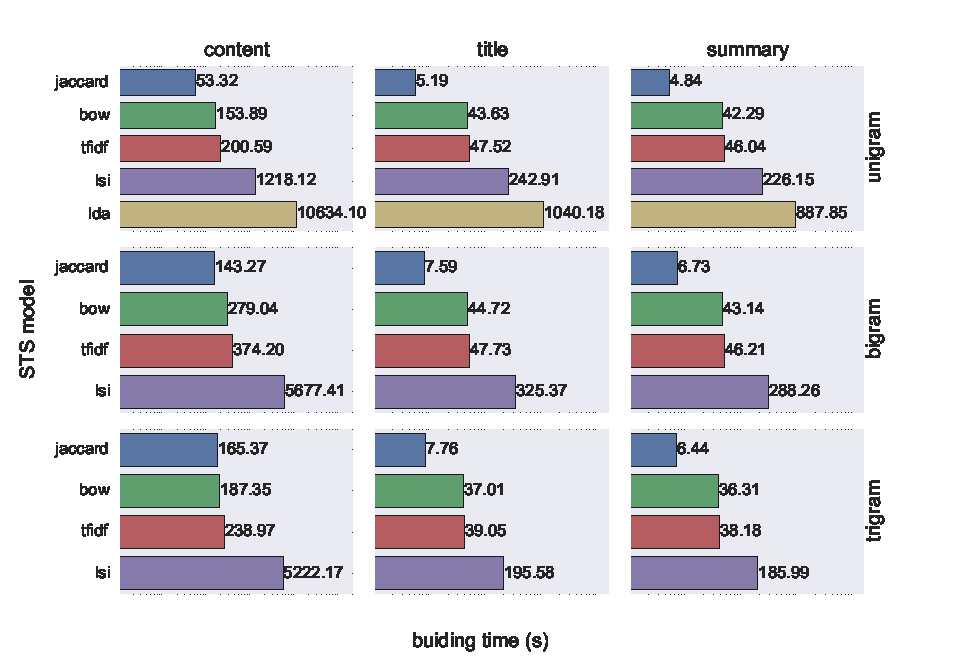
\includegraphics[width=\textwidth]{fig/building_time}
    \caption{Time cost of building phase}
    \label{fig:build_time}
\end{figure}

\begin{itemize}


\item Building phase of jaccard spends less time than other VSMs. Unlike VSMs, there is no model as ``middleware'' between articles and representation for jaccard. The building phase of jaccard is actually the phase where one article is reduced as a set of appeared terms. 

\item The building time cost of BoW and tdidf is roughly the same and tfidf spends slightly more time than BoW, because tdidf extends BoW with computing tf-idf weight. 

\item Topic models are more expensive. To be specific, LSI consumes more than 5 times for \icontent{} in unigram and even more than 20 times as much as the time tfidf consumes because of computing SVD. More seriously, the building time of LDA is 47 times as high as the building time of tfidf for \icontent{} in unigram and the time cost exceeds an acceptable range in bi- and trigram. 

\item Compared with unigram, the building time cost of jaccard, BoW, tfidf, LSI for \icontent{} in bigram, is increased by 3.2 times, 2.1 times, 2.1 times and 4.6 times, respectively, where as the time cost increases by only 2.4 times, 1.2 times, 1.2 times and 4.2 times correspondingly. On the other hand, the time cost of a particular STS model is not significantly different between uni-, bi- and trigram.

\end{itemize}

\subsubsection{Comparison of predicting time}

The results of predicting time are illustrated in figure \ref{fig:predict_time} and analyzed as follows. 
\begin{figure}[!htb]
    \centering
    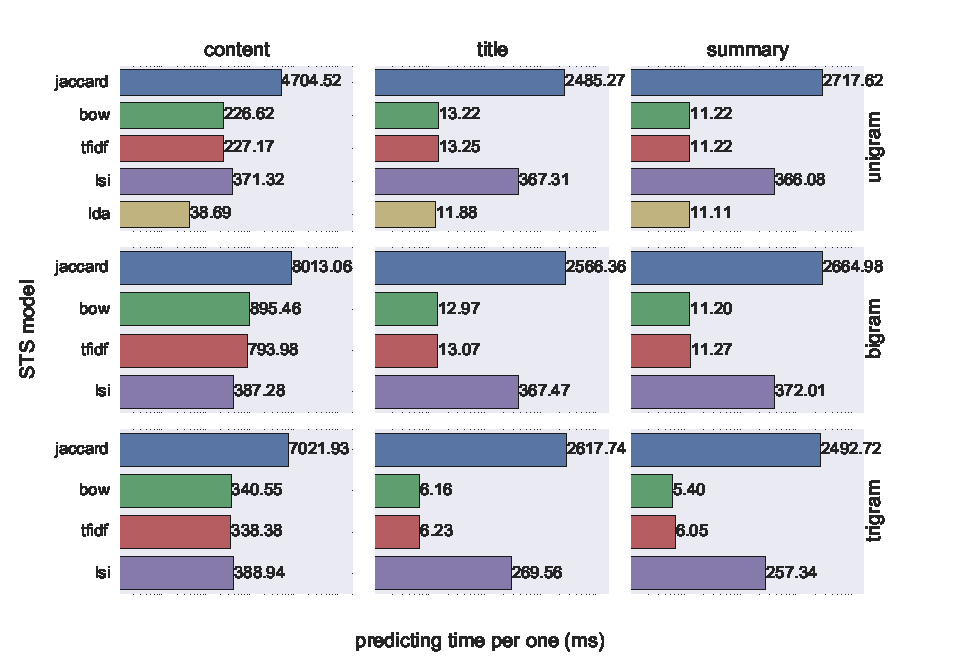
\includegraphics[width=\textwidth]{fig/predicting_time}
    \caption{Time cost of predicting related articles for one target}
    \label{fig:predict_time}
\end{figure}

\begin{itemize}
\item Similar to building phase, jaccard is also quite different from other VSMs. The jaccard similarity between two documents is computed by dividing the size of union of the corresponding term sets by the size of intersection of them. This operation is more costly than computing \textit{cosine} similarity between vectors. As compared with tfidf, jaccard costs 20-fold, 10-fold and 21 fold time for \icontent{} in uni-, bi- and trigram, respectively.

\item Predicting phase consists of representing phase and similarity computing phase. The first phase depends on the complexity of the corresponding model. Specifically, a document is represented as a vector of occurrence frequency, tf-idf weight and topic weight for BoW, tfidf and topic modles(i.e. LSI and LDA), respectively, and complexity increases progressively. The second phase depends on the vector dimension and the amount of vectors. Normally, the vector dimension of topic models is much lower than BoW and tfidf and hence, topic models cost less time in the second phase. In \icontent{}, the cost of LSI is similar to BoW and tfidf, whereas it is much higher than BoW and tfidf in \ititle{} and \isummary{}, which generate much smaller vocabularies and accordingly the lower vector dimension. 

\end{itemize} 

In conclusion, we determine the final selection of the best model for each dataset in table \ref{tab:select}, taking into account both of effectiveness and efficiency.

\begin{table}[!htb]
\centering
\begin{tabular}{|c|c|c|c|}
\hline
\textbf{Model} & \textbf{Content} & \textbf{Title} & \textbf{Summary} \\ \hline
\textbf{Unigram} & tfidf & tfidf & tfidf \\ \hline
\textbf{Bigram} & tfidf & tfidf & jaccard \\ \hline
\textbf{Trigram} & tfidf & jaccard & jaccard \\ \hline
\end{tabular}
\caption{Model selection for each data source in n-gram.}
\label{tab:select}
\end{table}

\clearpage

\subsection{Results of Incremental Updating}
\label{sec:5.4}

As described in section \ref{sec:4.4}, the whole corpus is splitted into a historic dataset, in which the articles are released before 2012 and which is used for initializing the system, and a testing dataset containing the released after 2012 articles, which is used for both of evaluating the system and updating the system incrementally. In the sight of reality, the candidates of related articles for a target article must be released before the target. We have two main purposes of the experiment. On the one hand, we attempt to find the differences between the results of the system with incremental updating and the results of the controlled experiments and analyse whether the differences are acceptable and the reason why the differences occur. On the other hand, we focus on the trade-off between the step of updating and the corresponding additional cost of time. 

Before analyzing the results, we define the controlled experiments in advance. The system in the controlled experiments is constant. It means, the systems are trained only in the phase of initialization and keep constant after that. In the first experiment, the STS methods in the system is learned from the candidate corpus, or, in other words, the released before 2012 articles. Accordingly the system contains only the semantic information before the first target is released and this system is hence ``out-of-date''. The system 1 is called the ``lower bound'' system. In the second experiment, there is only one difference from the first experiment, that the STS methods are trained by the all complete articles and the system contains therefore the complete semantic information of the entire corpus. The second controlled system is a ``upper bound'' system. Any article which is released before the target is transformed as the corresponding representation by the STS methods.  The comparison between the evaluated system and the controlled systems is able to indicate the particular characteristics of the system with incremental updating and the differences from the ``out-of-date'' system and ``coverall'' system. 

Jaccard and BoW are not involved in the evaluation. These two methods are only dependent on the current articles and independent of the rest information of the corpus. The model updating therefore does not affect the results of the semantic similarity from Jaccard and BoW. Consequently, the evaluation concentrates on three VSMs, namely tf-idf and LSI (due to the high complexity and low performance, LDA is ignored). Based on the result of experiment 1, the preprocessed field \icontent{} with unigram always outperforms other preprocessed fields. In this experiment, we only discuss the performance of the three STS methods in \icontent{} with unigram. 

\subsubsection{Effectiveness}

Instead of \textit{precision@k@h} used in experiment 1, we compute the precision with moving average, which is often applied with time series data to smooth out short-term fluctuations and highlight longer-term trends or cycles. A typical application of moving average is to analyze stock prices. In our case, we calculate the moving mean precision (MMP) of the $i$-th target article and $n-1$ previous targets mathematically as follows:

\begin{equation}
    MM_{i} = \frac{\sum^{n-1}_{j=0} \text{correct predictions for }(i-j)}{k\times n}
\end{equation}
where $n$ is the moving window size and pre-defined as $100$ and $k$ is the number of related articles for each target. 

\paragraph{Comparison with Controlled Systems}.

\begin{figure}[!htb]
    \centering
    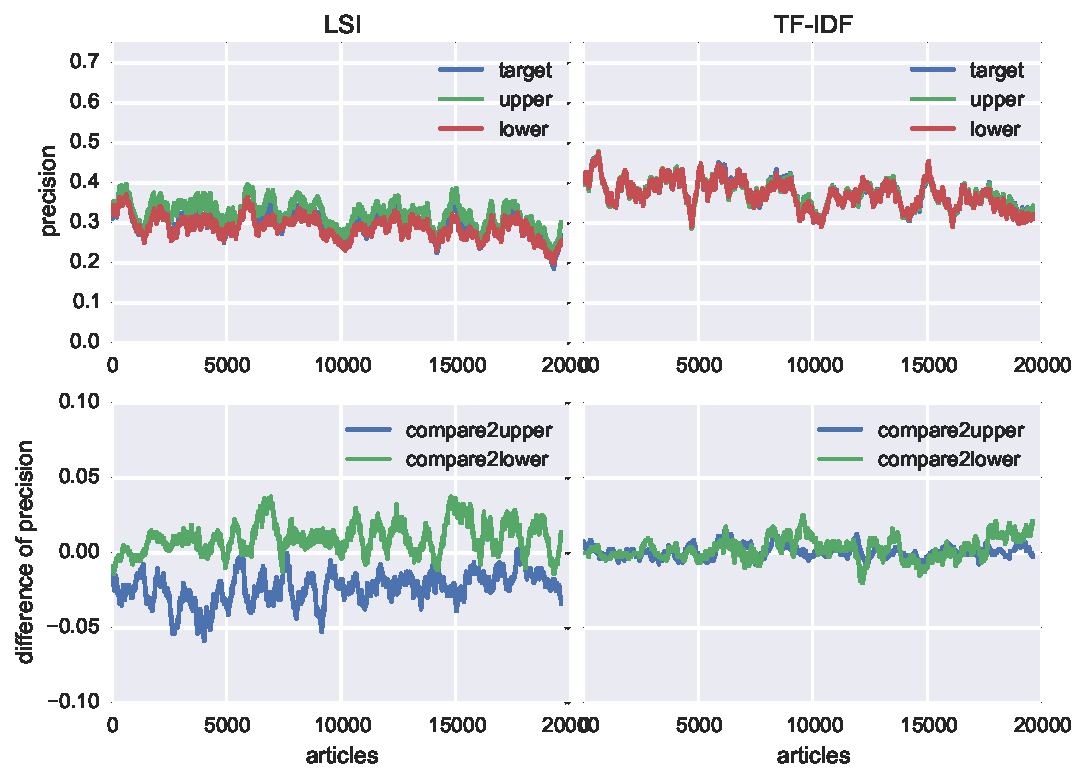
\includegraphics[width=\textwidth]{fig/precision_inc}
    \caption{Compare the precision of the evaluated system with the controlled systems. The window size of moving average is set to $400$.}
    \label{fig:predict_inc}
\end{figure}

Figure \ref{fig:predict_inc} illustrates the moving average precision which the evaluated system and the controlled systems achieve. In general, the average precision of the system using LSI and \tfidf{} is $29.95\%$ and $37.50\%$, respectively. The result confirms the conclusion we obtain in experiment 1. The subfigures below is obtained by subtracting the precision of the controlled systems from the precision of the evaluated system. For method LSI, the evaluated system outperforms the ``lower bound'' system and underperforms the ``upper bound'' system definitely. Meanwhile, the differences in the systems using \tfidf{} are insignificant. Therefore, LSI is more sensitive than \tfidf{} to the completeness of information and model updating. However, an interesting point for LSI is that the difference between the evaluated system and the ``lower bound'' system does not keep increasing or decreasing along with handling more and more articles, but the difference between the evaluated system and the ``upper bound'' system is in the increasing trend. 


%1. 不同methods的precision的变化曲线的横向对比:与实验一结论一致,但是precision低于实验一,主要原因可能是实验二只比较早于自己release的articles,number of related articles比实验一少,所以命中率低。
%2. 同一个method的precision与非增量算法得到的precision、每个article拥有的related articles数量曲线、模型更新点做纵向对比:incremental方法的precision略低于non-incremental,但是曲线形状基本一致;同时也与no. related articles一致,在模型更新之后delta-precision下降,随着模型的过时,delta-precision上升。

\paragraph{Correlation with the number of true related articles}

\paragraph{Impact of updating}


\subsubsection{Efficiency}

1. 总体来说,predicting的时间随着corpus的增加呈现线性递增,大概每100个articles增加xx\%;building时间也是线性递增,增长率为:
2. 在两次update之间,predicting时间呈现一个较高比率的增加,平均值为:而在update之后,时间则回落到正常值,主要原因是需要构建额外的matrix来计算similarity,这个可能是可以优化的空间。
3. 对于tfidf, bulding predicting时间比值平均为1.1 而lsi此比值为4.3。当然这个时间是dependent on update频率。 明显lsi所需要的building时间要更大。 考虑单次update的情况,这个占比是随着corpus的不断增长而有较为缓慢的下降的,也就是说predicting的时间的增长率要比building的时间增长率高。

\subsection{Error Analysis}
\label{sec:5.5}

We present insights on the most severe types of errors of false positive and false negative that occurred in the experiments. In order to confirm the reasons or conditions of the errors, we inspect manually the predictions of the framework to discover related articles and compare them with the golden standard understanding of human beings.  

\subsubsection{False Positive Error}

A false positive error is a result that indicates a given condition has been fulfilled, when it actually has not been fulfilled. In our case, a false positive error is the event that an article which is actually unrelated to the target article is assigned as related by the framework. 

\begin{itemize}
    \item One type of fp errors is caused by the labeled corpus we select. The list of related articles is marked by the editor manually and the size is limited up to $2$. Therefore, the list is incomplete, so that articles which should be related to each other under human understanding are unreachable to each other in the related-graph generated based on the lists of related articles. Only this type is not the real errors but the inherent systematic lack. 
    
    Example: 
    \begin{itemize}
        \item \textit{``Tod dem Diktator'' - Rufe zur Vereidigung} (\textit{``Death to the dictator'' - require for swearing}) \footnote{\url{http://www.zeit.de/online/2009/32/iran-proteste-vereidigung}}
        \item \textit{Proteste in Teheran dauern an} (\textit{Protests in Tehran persist}) \footnote{\url{http://www.zeit.de/online/2009/32/iran-ahmadineschad-proteste}}
    \end{itemize}
    The both articles report the protest against Mahmoud Ahmadinejad, who is re-elected as the Iranian president, and the international as well as authoritative reaction. The articles should be related by the human judgement, but there is no related-path between them. We consider that the incompleteness of labeling causes the fp error. 
    
    \item One article usually contains a set of topics rather than the single topic. The topics are not treated equally, but they are understood in different importance. It is complicate and subtle, how human beings weigh the importance of different topics. Out of this view point, two articles are assigned as related, only when they share the topics with the highest weight, otherwise they are unrelated, even though they are similar to each other in semantic or lexical meaning. 
    
    Example:
    \begin{itemize}
        \item \textit{Tunesiens Innenminister wird neuer Regierungschef} (\textit{Tunisia Interior Minister appointed new head of government}) \footnote{\url{http://www.zeit.de/politik/ausland/2013-02/tunesien-regierungschef-larayedh-jebali}}
        \item \textit{Tunesien hebt den Ausnahmezustand seit Arabellion auf} (\textit{Tunisia cancels the state of emergency beginning from Arabellion}) \footnote{\url{http://www.zeit.de/politik/ausland/2014-03/tunesien-ausnahmezustand-aufhebung}}
    \end{itemize}
    
    The both articles mention the identical background, subject of the events and keywords. However, the critical reported topics are different and unrelated. In addition, quite a few named entities which they share confuse the framework predicts the relatedness between them. 
    
    \item Two articles have the identical or similar information, but they mention the very different topics. 
    Example: 
    \begin{itemize}
        \item \textit{Dem Pr\"asidentenpaar droht eine herbe Wahlniederlage} (\textit{The presidential couple threatens a bitter election defeat}) \footnote{\url{http://www.zeit.de/online/2009/27/argentinien-wahl-kirchner}}
        \item \textit{Der Schattenpr\"asident} (\textit{The Shadow President}) \footnote{\url{http://www.zeit.de/politik/ausland/2010-10/nestor-kirchner-nachruf}}
    \end{itemize}
    The articles report the politics in Argentina and use many similar or same words to describe the situation of the government and the action thereof. However, the first article focuses on the difficulty of election, while the second article reviews mainly the record of achievements of the former president who just died. Hence, they are unrelated very clearly. 
    
    \item Two articles are about entirely different field and totally unrelated. 
    
    Example: 
    \begin{itemize}
        \item \textit{Ohne Gras kein Spa\ss{}} (\textit{Without grass no fun}) \footnote{\url{http://www.zeit.de/2009/20/Portugal-Golf}}
        \item \textit{Jonglieren entspannt und macht schlau} (\textit{Juggling relaxed and makes you smart}) \footnote{\url{http://www.zeit.de/karriere/beruf/2012-10/konzentration-gehirnleistung-jonglage}}
    \end{itemize}
    
    The first article describes the experiences of the golf trip in Portugal, whereas the second article reports a kind of game in office which can make the participants relaxer and smarter. They belong to even different separated categories and cannot be related to each other. 
\end{itemize}

\subsubsection{False Negative Error}

A false positive error is, in our case, a result that indicates an article which is actually quite related to the target article is judged with a very low relatedness degree. Now we consider that the articles which are very related to the target article are exactly predicted unrelated with an unexpected low relatedness degree. More specifically, we only inspect the extreme and typical error that the framework treats the articles which are directly adjacent to the target article in the related-graph and should be one of the most related articles as unrelated in a very low level. We discuss the characteristics of the errors and the reasons why the errors occur. 

\begin{itemize}
    \item Two articles discuss the same topics and related meaning, but the points of view and concrete events are different. 
    
    Example:
    \begin{itemize}
    \item \textit{Drittmittel sind ungleich verteilt} (\textit{Third-party funds are distributed unequally}) \footnote{\url{http://www.zeit.de/studium/hochschule/2014-02/Drittmittel-an-Hochschulen}}
    \item \textit{Uni Leipzig droht mit Schlie\ss{}ung ganzer Fakult\"aten} (\textit{Uni Leipzig threatened with closure of entire faculties}) \footnote{\url{http://www.zeit.de/studium/hochschule/2014-02/universitaet-leipzig-finanzierung}}
    \end{itemize}
    The first article discusses the phenomenon of education abstractly, while the second reports the very concrete expression in a specific university. They are not similar semantically, but related because of the same topic.
    
    
    \item Humans classify an articles into topics hierarchically rather than separately. Two articles may be related in higher level but different in the particular level. The critical point is how the humans determine which level is the most important. 
    
    Example:
    \begin{itemize}
        \item \textit{Der Jugendschutzfilter blockiert zu viel} (\textit{The youth safety filter blocking too much}) \footnote{\url{http://www.zeit.de/digital/internet/2012-02/jugendschutzfilter-filtern-blogs}}
        \item \textit{Filmwirtschaft weitet Selbstkontrolle auf Internet aus} (\textit{Film industry is expanding self-regulation on the Internet}) \footnote{\url{http://www.zeit.de/kultur/film/2011-10/fsk-jugendschutz-internet}}
    \end{itemize}    
    
    The first article reports the current situation of the youth safety filter and the second article reports that the change of film industry on the Internet may harm the youth protection. These two article share the same topic on ``youth procection'' but have difference on the particular fields. They are labeled as related based on the editor's understanding. However, this judgement is not absolutely correct. 
    
\end{itemize}


%\subsection{Conclusion}
%\label{sec:5.6}
%1. 分析了性能,分析了错误
%2. 最好的是content-1-tfidf,其他的见表格
%3. 问题是没有使用corpus中的标记,即保存的人工标记related。利用这些数据,会训练出更加specific更加precise的模型,在下一章详细说明。
  \clearpage
  \section{Combination Approaches}
\label{sec:6}

In this section, we focus on applying supervised methods for improving the effectiveness of the system. In subsection \ref{sec:6.1} the motivation and feasibility of using supervised methods are interpreted. After that, we describe the additional features besides the results from the STS methods in subsection \ref{sec:6.2}. After a brief introduction of the selected supervised methods in subsection \ref{sec:6.3}, the results of experiments which are evaluated using such methods are reported in subsection \ref{sec:6.4}. In addition, the best supervised method and the corresponding combination of features are concluded also in the subsection \ref{sec:6.4}.


\subsection{Motivation and Feasibility}
\label{sec:6.1}

First, the experiments which are reported in section \ref{sec:5} are designed to evaluate the performance of the single methods on a specific text field. In other words, the evaluated objects are the performance of the STS methods rather than the performance of the system. We attempt to find out a combination approach to let the system outperform the system using any single method. Second, the meta-data are totally disregarded in the previous experiments. However, the information of meta-data is useful to reinforce or undermine the relatedness degree between articles. For example, figure \ref{fig:release_relate} reports the accumulation of distribution of the release time interval of all related pairs and shows that the release time interval between $16\%$, $38\%$, $60\%$ and $85\%$ related-article-pairs is less than one week, one month, $100$ days and one year. From this it can be seen that an article intends to be more related to the one closer to it in term of the release time. Third, each article-pair has an integer label which indicates the relatedness degree. The label of $y=11 -h ~~(1 \le h \le 10)$ refers to the corresponding articles are related with an $h$-distance path in the related-graph and the label \textit{0} refers to the articles are unrelated. The labels can be used for training supervised methods to improve the performance of the system. 

The core task of our work is to select the articles which have the highest score. From the viewpoint of machine learning, the task is an application of learning to rank, but only the articles in the top position of the ranking are required. More detailed, for each target article, the system computes the scores for all target-candidate pairs. The two pairs with the highest scores are judged to be related to each other. The ``basic'' input object of training example of supervised methods is a set of features which are generated from a target-candidate pair, and the output object is a label which is extracted from the related-graph. We use the additional word ``basic'', because the input objects are different from the ``basic'' objects but based on them in pairwise and listwise methods. 

From the viewpoint of learning to rank, we rename several concepts and define the new notations being used in this section. In this section, we use the term ``query'' which refer to the concept ``target article'', but we also use ``candidates'' to indicate articles being related articles potentially. $\mathbf{x}_{i, j}$ refer to the basic feature vector which is extract from the pair of query $i$ and candidate $j$. $y_{i,j}$ is the label of example, which could be either $0$ or $1$ in the algorithms of binary classification or a ranking degree in the algorithms of information retrieval. $\mathbf{x}_{i,j}$. 

\begin{figure}[!htb]
    \centering
    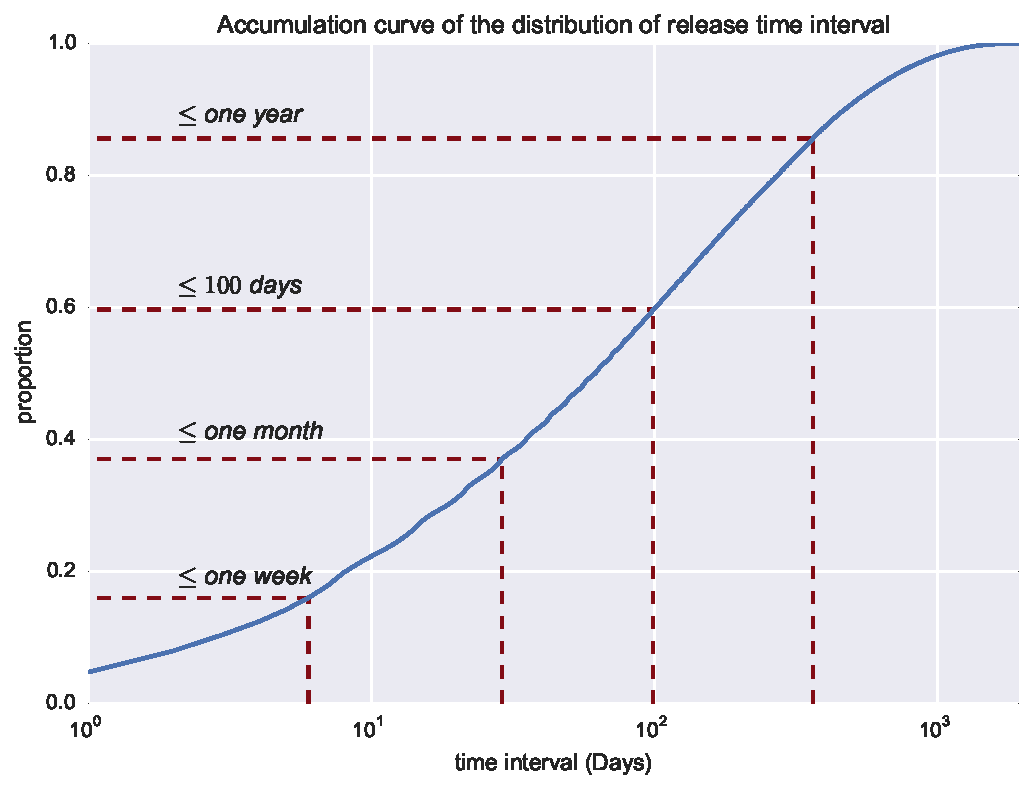
\includegraphics[width=0.8\textwidth]{fig/release_related}
    \caption{The accumulated distribution of the release time interval between any two related articles. }
    \label{fig:release_relate}
\end{figure}

\subsection{Feature Generation}
\label{sec:6.2}

Each feature is computed from the comparison of two articles in a specific attribute. The value range of each feature is normalized to the range between $0$ and $1$. One type of features is the semantic textual similarity over particular text fields, such as \tfidf{} similarity and LSI similarity over \icontent{}. Another type is the comparison of meta-data between articles. The computation of remaining features is defined as follows.

\paragraph{\texttt{category}}

This feature indicates the category relevance between two articles. Each article belongs to a category. Let $c_i$ denote the category which query $i$ belongs to and $c_j$ the category which candidate $j$ belongs to. We say the number of all categories is $n$. For each query $i$, the distribution of related categories which true related articles belong to. The $n\times n$ matrix of related categories is computed by adding distributions for all queries. The matrix is marked as $\mathbf{M}$, where $\mathbf{M}_{\alpha,\beta}$ refers to the corresponding category relevance between a query which belongs to category $\alpha$ and a candidate which belongs to category $\beta$. Hence, feature \texttt{category} of an query-candidate pair, $\langle i, j \rangle$ , is $\mathbf{M}_{c_i, c_j}$.

\paragraph{\texttt{keyword}}

This feature indicates the keyword relevance between query $i$ and candidate $j$. First, the inverse-document-frequency (\textit{idf}) of keyword $k$ is computed with $$idf_k=log_2 \dfrac{\text{the number of all candidates}}{\text{the number of candidates containing keyword}~~k}$$ Assuming a series of keywords $\mathbf{K}={k_1, \cdots, k_m}$ which occur in both of query $i$ and candidate $j$, we compute feature \texttt{keyword} with $\sum_{i=1}^{m} idf_{k_i}$. One issue of this feature is normalization. In our case, the feature value is divided by the greatest value in all examples of the corresponding query. 

\paragraph{\texttt{release time}} 

This feature indicates the relevance of issue time between query $i$ and candidate $j$. Let $r_i$ denote the release time of query $i$ and $r_j$ the release time of candidate $j$. The time interval $\Delta_{i,j}=\text{days}~(|r_i - r_j|)$. \\ With normalization, feature $\mathtt{release~time} = \begin{cases} \Delta_{ij}~/~365, & \Delta_{ij} < 365 \\ 1, & \Delta_{ij} \ge \text{one year} \end{cases}$. 

\paragraph{\texttt{term ratio}} 

This feature indicates the term relevance between query $i$ and candidate $j$. Let $v_i$ denote the vocabulary of query $i$ which is extracted from \icontent{} and $v_j$ the vocabulary of candidate $j$. Feature \texttt{term ratio} equals the ratio of the size of the smaller of the two vocabulary to the size of the larger one. 

\paragraph{\texttt{token ratio}} This feature indicates the length relevance between query $i$ and candidate $j$. Feature \texttt{token ratio} is the ratio of the number of tokens of the shorter of the two \icontent{} documents to the number of tokens of the longer one. 

Now we have $3$ so-called ``meta-data'' features including \texttt{category}, \texttt{keyword} and \texttt{release time} which are generated from meta-data, $2$ ``extended'' features including \texttt{term ratio} and \texttt{token ratio} which are extracted from the \icontent{}, and $11$ ``STS'' features which are reported in table \ref{tab:select}. In order to describe the STS features simply, each such feature is denoted by a short symbol. The symbol is in the format of \texttt{\{n\}\{f\}-\{m\}}, where \texttt{\{n\}} refers to an n-gram model and the possible values are $1$, $2$ and $3$, \texttt{\{f\}} to a text field, and \texttt{\{m\}} to an STS method. The possible assignments of \texttt{\{f\}} are \textit{c}, \textit{t} and \textit{s}, which present \icontent{}, \ititle{} and \isummary{}, respectively. \texttt{\{m\}} can be assigned with \textit{j}, \textit{t} and \textit{l} as the abbreviations of method Jaccard, \tfidf{} and LSI, respectively. For example, \texttt{1c-t} means the feature of the similarity score of method \tfidf{} for \icontent{} over unigram.


\subsection{Experimental Setup}
\label{sec:6.3}

The algorithms of learning to rank can be classified into the pointwise, pairwise and listwise approaches. First, in the pointwise approach, the algorithms are trained directly by the feature vector of each single candidate over the corresponding query, and the output is the relatedness degree. The pointwise approach hence does not distinguish different queries, and moreover, it can be treated as an application of the algorithms of binary or multiclass classification. Second, the input of an example in the pairwise approach is a feature vector which is computed by comparing the feature vectors of two query-candidate pairs with the same query, and the output is assigned from $\{0, 1\}$, where $1$ refers to the first candidate should be in the better position in the ranking than the second candidate for the mentioned query, and $-1$ refers to the contrary. The pairwise approach also ignores the difference of queries, and it can apply the algorithms of binary classification. The pairwise approach has the issue of computational complexity. There are $\frac{n(n-1)}{2}$ examples for an arbitrary query and a corpus of $n$ candidates. That is to say, the time cost of the learning and predicting phases increases quadratically. From this reason, the pairwise approach is discarded in the experiment. Third, the listwise approach uses a feature matrix as input of an example with combining the the feature vectors of all query-candidate pairs for an identical query. The output of the example is a series of relatedness degree or the ranking of candidates. In the listwise approach, the algorithms operate directly on the level of queries but not of candidates. 

Logistic regression and Multiple Additive Regression Tree (MART) \citep{friedman2002stochastic}, which are the algorithms of the pointwise approach, are selected. An algorithm of the listwise approach, ListNet \citep{cao2007learning}, is selected to evaluate. 

In logistic regression, the labels are assigned from $\{0, 1\}$ instead of relatedness degree. If the relatedness degree between the query and the candidate is greater than or equal to $3$, the candidate is related to the query and then the label is assigned with $1$, otherwise, with $0$. The output of logistic regression is the probabilities that the candidate is related to the query. The 2 candidates with the highest probability are selected as related articles. In MART and ListNet, the label of each example is the value of relatedness degree. 

\subsection{Experimental Results}
\label{sec:6.4}

\begin{table}[!hbt]
\centering
\resizebox{\textwidth}{!}{%
\begin{tabularx}{1\textwidth}{lX|rr|rr|rr}
\multirow{2}{*}{\textbf{No.}} & \multirow{2}{*}{\textbf{Feature Set}}  & \multicolumn{2}{c|}{\textbf{LogReg}} & \multicolumn{2}{c|}{\textbf{MART}} & \multicolumn{2}{c}{\textbf{ListNet}} \\
\textbf{} & \textbf{} & \textbf{p@2@3} & \textbf{nDCG} & \textbf{p@2@3} & \textbf{nDCG} & \textbf{p@2@3} & \textbf{nDCG} \\ \hline
\#00 & 1c-t (BASELINE) & 0.440 & 0.722 & 0.440 & 0.722 & 0.440 & 0.722 \\ \hline
\#01 & 1c-t, 1c-l & 0.458 & 0.728 & 0.445 & 0.726 &  0.453 & 0.727\\
\#02 & 1c-t, 1c-l, 1t-t, 1s-t & 0.468 & 0.731  & 0.473 & 0.732  & 0.465 & 0.731\\
\#03 & 1c-t, 1c-l, 2c-t, 3c-j & 0.485 & 0.732 & 0.464 & 0.728 & 0.481 & 0.733\\
\#04 & all features & 0.489 & 0.735 & 0.487 & 0.734 & 0.493 & 0.734\\
\#05 & category + \#01 & 0.467 & 0.730 & 0.445 & 0.729 & 0.460 & 0.728\\
\#06 & category + \#02 & 0.470 & 0.734 & 0.471 & 0.735 & 0.432 & 0.725\\
\#07 & category + \#04 & 0.492 & 0.738 & 0.487 & 0.736 & 0.460 & 0.726\\
\#08 & keyword + \#01 & 0.475 &  0.732 & 0.464 & 0.730 & 0.482 & 0.733\\
\#09 & keyword + \#02 & 0.494 & 0.735 & 0.476 & 0.735 & 0.480 & 0.732\\
\#10 & keyword + \#04 & 0.508 & 0.739 & 0.490 & 0.736 & 0.495 & 0.737\\
\#11 & release + \#01 & 0.617 & 0.769 & 0.590 & 0.769 & 0.628 & 0.767\\
\#12 & release + \#02 & 0.623 & 0.772 & 0.609 & 0.773 & 0.615 & 0.770\\
\#13 & release + \#04 & 0.630 & 0.773 & \textbf{0.622} & 0.773 & 0.588 & 0.763\\
\#14 & meta-data + \#01 & 0.629 & 0.774 & 0.593 & 0.775 & 0.598 & 0.763\\
\#15 & meta-data + \#02 & \textbf{0.640} & \textbf{0.778} & 0.599 & 0.776 & \textbf{0.637} & \textbf{0.774} \\
\#16 & meta-data + \#04 & 0.635 & 0.777 & 0.619 & \textbf{0.779} & 0.633 & 0.773\\
\#17 & meta-data + extend-data + \#01 & 0.628 & 0.774 & 0.587 & 0.774 & 0.605 & 0.767\\
\#18 & meta-data + extend-data + \#02 & \textbf{0.640} &  0.777 & 0.605 & 0.777 & 0.608 & 0.769\\
\#19 & meta-data + extend-data + \#04 & 0.634 & 0.777 & 0.612 & \textbf{0.779} & 0.585 & 0.767 \\ \hline
\end{tabularx}
}
\caption[\textit{Precision@2@3} and \textit{nDCG} of logistic regression, MART and ListNet with the different selections of features in 5-fold cross validation]{\textit{Precision@2@3} of logistic regression (abbr. LogReg), MART and ListNet with the different selections of features. The baseline feature is the scores generated by the best system with method \tfidf{} for \icontent{} over unigram. Feature set ``meta-data'' includes features \texttt{category}, \texttt{keyword} and \texttt{release time} and ``extend-data'' includes \texttt{term ratio} and \texttt{token ratio}}
\label{tab:supervised}
\end{table}


The supervised system is evaluated using 5-fold cross-validation. The final system with the average parameters or coefficients is available to compute the relatedness scores for testing query-candidate pairs and discover related articles for the corresponding query. We configures $19$ feature sets with different combination between meta-data, extend-data and STS features to train the three algorithms  respectively. In addition, we choose the effectiveness of the system using \tfidf{} in \icontent{} over unigram (1c-t) as the baseline, because the system has the best effectiveness in all unsupervised systems with single STS method. 

Table \ref{tab:supervised} reports the configuration of feature sets and the results that each algorithm performs with these feature sets. For logistic regression, the system using feature set \# 15 has both of the best \textit{precision@2@3} of $0.640$ and \textit{nDCG} of $0.778$. Feature sets, \# 18, \#16 and \#19, has slightly worse performance than \#15 and take separately the second place to the fifth place. ListNet, which uses a linear Neural Network model, has the similar results to logistic regression. For ListNet, \#15, \#16, \#11 take respectively the first, second and third place. For MART, which applies regression trees, feature set \#13 trains the best performed algorithm in \textit{precision@2@3} but the best result of \textit{nDCG} is obtained from \#16 and \#19. MART has the greatest different between \textit{precision@2@3} and \textit{nDCG} in the identical feature set. Hence, MART is the most unstable algorithm in the experiment. The one result of the experiment is that the system using logistic regression outweighs the systems using MART and ListNet.


\begin{table}[!hbt]
\centering
\begin{tabularx}{0.8\textwidth}{lXrr}
\textbf{Feature} & \textbf{Description}  & \textbf{Coef in \#15} & \textbf{Coef in \#19} \\ \hline
1c-t & \tfidf{} in \icontent{} for unigram     & $+~3.036$  & $+~3.045$     \\
release & release time relevance & $-~2.235$   &  $-~2.231$     \\
keyword & keyword relevance  & $+~1.318$  & $+~1.322$ \\
1c-l & LSI in \icontent{} for unigram     & $+~1.260$   & $+~1.264$    \\
1t-t & \tfidf{} in \ititle{} for unigram     & $+~1.073$   & $+~1.073$      \\
category & category relevance & $+~0.907$   & $+~0.918$     \\
1s-t & \tfidf{} in \isummary{} for unigram      & $+~0.554$   & $~+0.554$     \\ \hline
token ratio & - & - & $-~0.042$ \\ 
term ratio & - & - & $-~0.025$ \\ \hline
\end{tabularx}
\caption[The feature coefficients for logistic regression in settings \#15 and \#19 which perform better than other combinations of algorithms and feature settings]{The feature coefficient for logistic regression in settings \#15 and \#19 which perform better than other combinations of algorithms and feature settings. The coefficients are ranked in descending order of the absolute value. }
\label{tab:coef}
\end{table}


\begin{figure}[!htb]
    \centering
    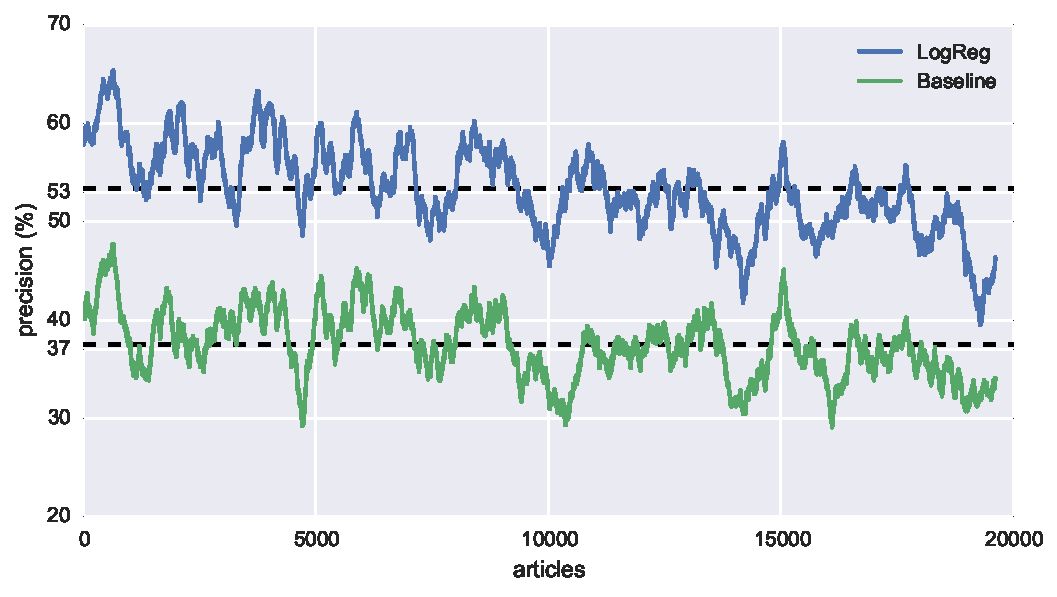
\includegraphics[width=\textwidth]{fig/precision_inc_supervised}
    \caption[]{}
    \label{fig:prec_supervised}
\end{figure}
  \clearpage
  \section{Conclusion}

The intention of this work is to design the system to discover related articles in a large corpus automatically and evaluate the performance and usability thereof. We use \textit{Semantic Textual Similarity} (STS) methods as the main methods to quantify the relatedness degree between two articles. After the algorithms being to evaluate are selected, the different text fields in articles are also to evaluate. Therefore, the basic configuration of the system is the combination of an algorithm and a (preprocessed over n-gram) text field. We evaluate the effectiveness and efficiency of systems. Effectiveness which includes \textit{precision@2@3} and \textit{nDCG} is the measure of the quality of the outputted results of systems. Efficiency is the measure of the cost of resource (e.g. operational time) during running of systems to discover related articles. 

We setup the experiments to test the performance of static and dynamic systems using different combination of algorithms and text fields. ``Static'' means the corpus of articles is constant during the experiment. ``Dynamic'' means the corpus keeps increasing in running of systems, that is to say, once a target article have ``obtained'' related articles from systems, it is inserted immediately into the corpus as candidates of potential related article for future articles. The static experiment is used for comparing the performance of different STS methods in different text fields and the dynamic experiment focuses on the influence of the increasing corpus on the performance of systems. 

All STS methods are unsupervised and document-based, and hence the labels of training data and the information in meta-data are not utilized. In the viewpoint of the supervised approach, it is regarded as an application of learning to rank in the field of Information Retrieval. Therefore, the algorithms on learning to rank, such as logistic regression and ListNet, are set up on the base of the existed system to make full use of all kinds of data including meta-data and STS scores as features and improve the usability of the system.


\subsection{Answer of Research Question}

In this part, we summarize this work by way of answering the research questions which are raised in section \ref{sec:2.5}. 

\paragraph{Can Semantic Text Similarity including string-based and vector space models methods be used for finding related articles? How effective and efficient is the metrics of performance, such as precision and operational time?}

The former sub-question can be answered positively in section \ref{sec:5.3}. The system using \tfidf{} in text field \icontent{} over unigram has the best effectiveness with \textit{precision@2@3} of $45.07\%$ (see figure \ref{fig:precision_2_3}) and the acceptable efficiency (figure \ref{fig:build_time} and \ref{fig:predict_time}). Finding related articles for one target costs on average $340ms$\footnote{}, if the time of system building is taken into account.  

\paragraph{How do the methods work in the practical scenario that the corpus keeps increasing with time? How is the performance of the incremental system different from a constant system? }

From the results of the second experiment which are reported in section \ref{sec:5.4}, the STS methods work also well in the increasing candidate corpus. The effectiveness is better than the so-called ``out-of-date'' controlled system which is never updated in running and meanwhile worse than the other so-called ``coverall'' controlled system which is trained by the historical articles and future articles. In terms of efficiency, the time cost of system updating and predicting also increases linearly during corpus increasing. 


\paragraph{Is it useful to combine the STS methods? Does it yield to an improvement in performance?}

The question could be answered relative negatively due to the results in section \ref{sec:6.4}. The effectiveness of combinations (\#1, \#2, \#3 and \#4) of the STS methods is slightly higher than the system using the best single STS method. Therefore, combing the STS methods cannot lead to a significant improvement in performance. 

\paragraph{The above introduced methods are unsupervised and ignore other meta-data. Does it lead to an improvement with utilizing supervised or semi-supervised algorithms which are proposed in the field of learning to rank?}

The question can be answered positively also in section \ref{sec:6.4}. Logistic regression with the feature set of meta-data and the best STS methods over unigram yields to the highest improvement in effectiveness. The \textit{precision@2@3} of this system is $64.0\%$ and improved by $20.0$ percent compared with the baseline in the static experiment. On the other hand, the final system has the average \textit{precision@2@3} of $53.38\%$ and outperforms the baseline by $15.86$ percent. 

\subsection{Application in Reality}
如果将系统实际使用,考虑到现在可以达到的准确率,无法实现完全自动化,可选取五个作为备选,然后人工选择,这一操作也可以大大提高准确率和减少工作量。


\begin{figure}[!htb]
    \centering
    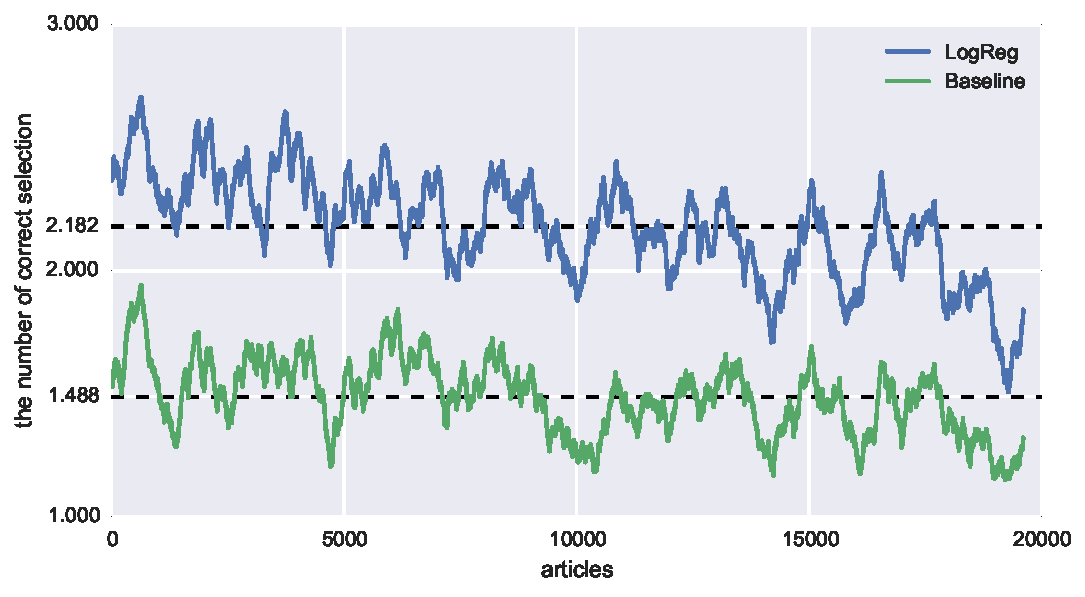
\includegraphics[width=\textwidth]{fig/precision_inc_supervised_5}
    \caption[]{}
    \label{fig:top5}
\end{figure}

\subsection{Future Work}
首先说明系统设计中的lack,即存在比较大的bias,因为我们主观的将discover related articles的过程简化为计算STS并combine with meta-data relevance. 这个做法会产生较大的bias, errors are reported in section 5. Future work 是可以使用其他的附加方法,来减少或者消除bias,在更精确的同时,达到覆盖更恰当的范围。

  \clearpage
  
  
  \medskip
\addcontentsline{toc}{section}{Bibliography}

\bibliographystyle{apalike}
\bibliography{cites}
\end{document}
